
\documentclass{beamer}

\usepackage{algpseudocode, color, colortbl, listings, MnSymbol}

\usepackage{hyperref}
\hypersetup{
    colorlinks=true,
    urlcolor=blue,
}

\usetheme{Montpellier}
\usecolortheme{rose}

% page numbers, from
% https://tex.stackexchange.com/questions/137022/how-to-insert-page-number-in-beamer-navigation-symbols
\expandafter\def\expandafter\insertshorttitle\expandafter{%
  \insertshorttitle\hfill%
  \insertframenumber\,/\,\inserttotalframenumber}

\definecolor{Gray}{gray}{0.8}
\newcolumntype{g}{>{\columncolor{Gray}}c}

\newcommand{\stanza}{ \\~\ }

\title{14. Approximation, Vertex Cover, and TSP}
\subtitle{CPSC 535}
\author{Kevin A. Wortman}
\institute{ 
\includegraphics[height=2cm]{csuf-logo-cmyk} }
\date{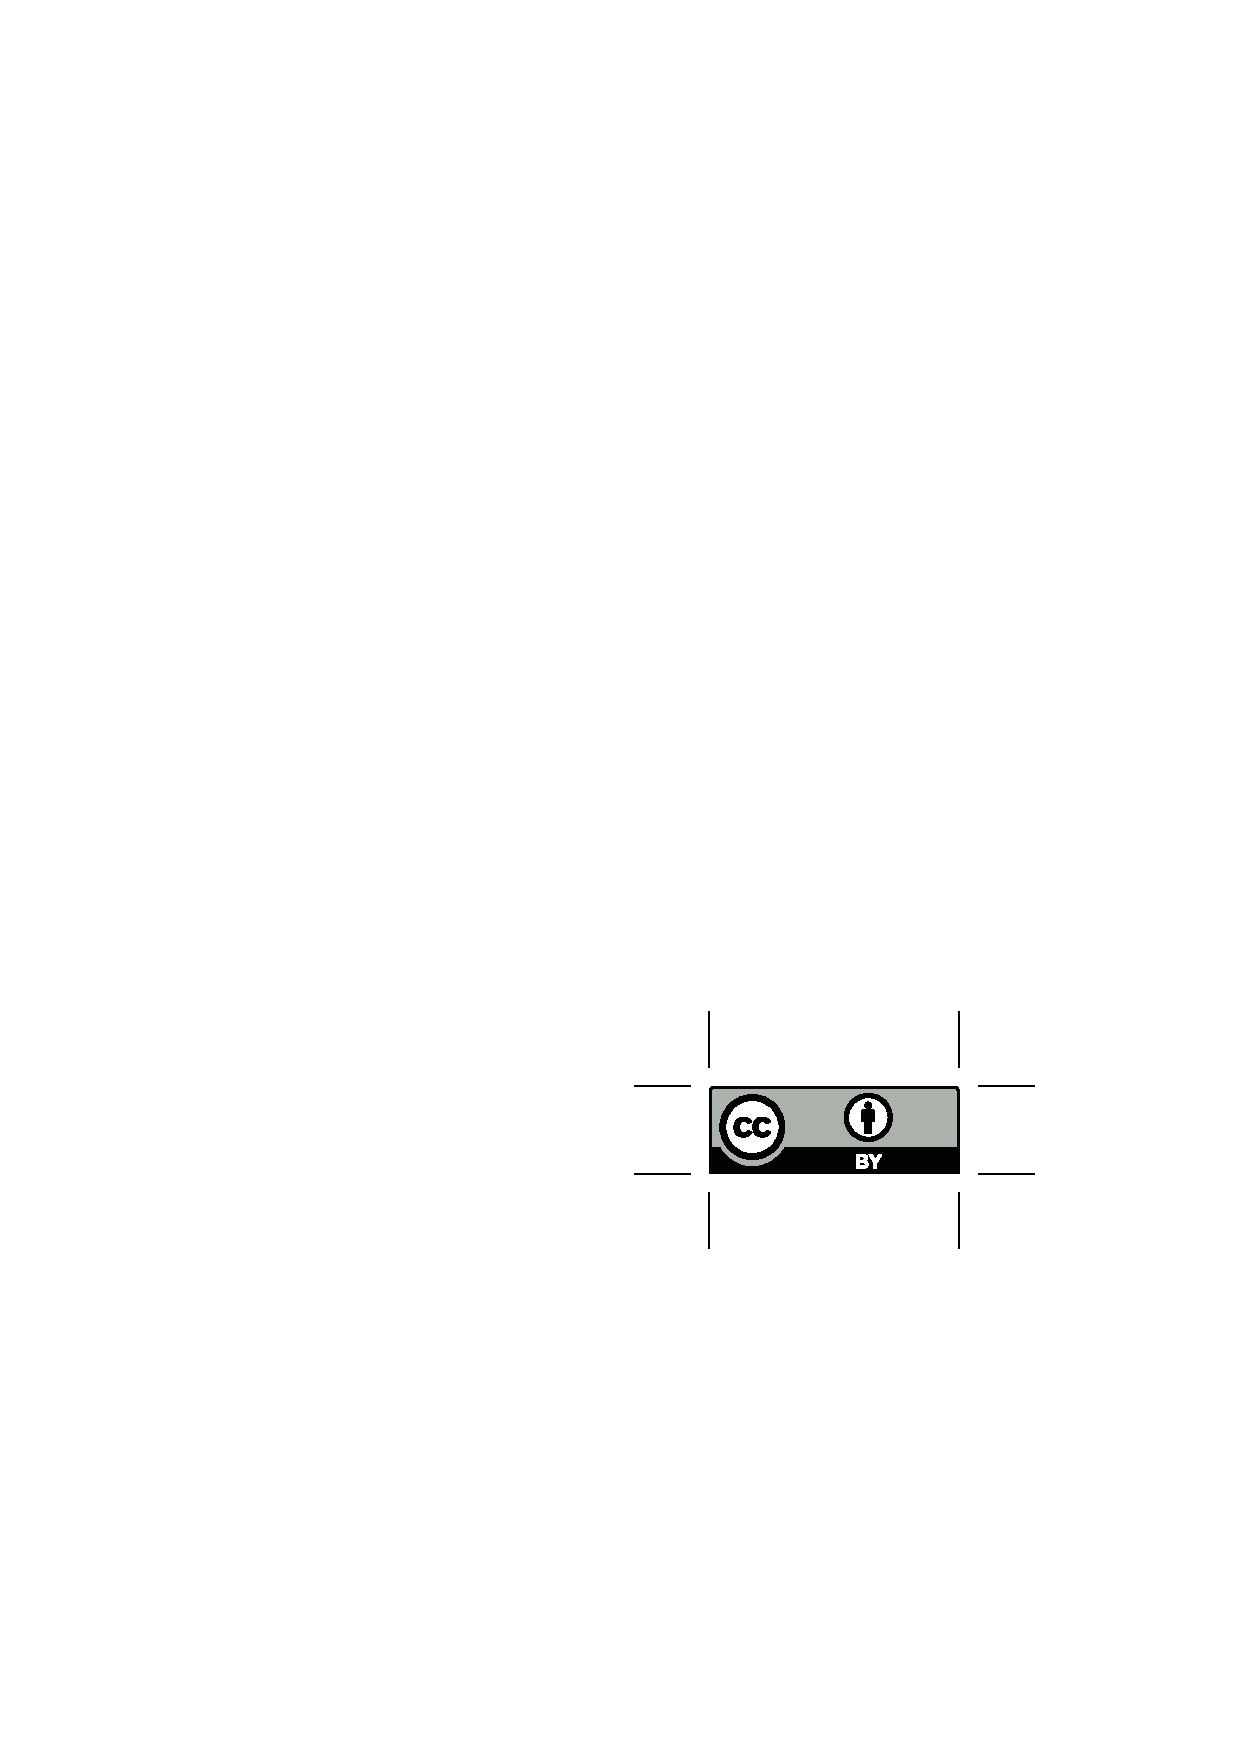
\includegraphics[height=14pt]{by} \\

{\tiny
This work is licensed under a
\href{http://creativecommons.org/licenses/by/4.0/}{Creative Commons Attribution 4.0 International License}.
}}

\begin{document}

\begin{frame}
  \titlepage
\end{frame}

\begin{frame} \frametitle{Big Idea: Renegotiating Problems}
Sometimes we want to solve a problem, but there is an obstacle
\begin{itemize}
  \item computational complexity: problem is $NP$-hard or undecidable
  \item ill-posed: don't know how to phrase problem as precise input/output statement
  \stanza
\end{itemize}

These are insurmountable; progress is impossible.
\end{frame}

\begin{frame} \frametitle{Big Idea: Renegotiating Problems}
  Sometimes we can \emph{negotiate} on the definition of the problem
\begin{itemize}
  \item adjust input/output def'n to correspond to an easier problem
  \item more specific input
  \item or, more general output
  \item ideally, still helps with the domain problem
  \item combines CS hard skills with domain soft skills
\end{itemize}
\end{frame}

\begin{frame} \frametitle{Approximation}
\textbf{Approximation}: output is \emph{nearly-optimal} but not necessarily
truly optimal.
\begin{itemize}
  \item quality is quantified, \textbf{proven}
  \item ``approximation'', ``approximate'' are technical terms; use other words
    like ``decent'' for informal ideas about quality
  \item suitable for use cases where approximate solutions are adequate
  \item need to rewrite problem definition
  \item every optimization problem has corresponding approximation problems; but these
    are distinct problems
\end{itemize}
\end{frame}

\begin{frame} \frametitle{Example: optimal vs. approximate graph coloring}
\emph{graph coloring} \\
\textbf{input}: connected graph $G=(V,E)$ \\
\textbf{output}: coloring $c$ using $k$ colors, where each vertex $v \in V$ is assigned color
  $c(v) \in \{1, \ldots k\},$ no pair of adjacent vertices are assigned the
  same color, and the number of colors $k$ is minimal
\stanza

\emph{3-approximate graph coloring} \\
\textbf{input}: connected graph $G=(V,E)$ \\
\textbf{output}: coloring $c$ using $k$ colors, where each vertex $v \in V$ is assigned color
  $c(v) \in \{1, \ldots k\},$ no pair of adjacent vertices are assigned the
  same color, \textbf{and the number of colors $k$ satisfies $k \leq 3 k^\star$,
  where $k^\star$ is the fewest colors possible for $G$}
\end{frame}

\begin{frame} \frametitle{Graph Coloring Example}
  \begin{center}
    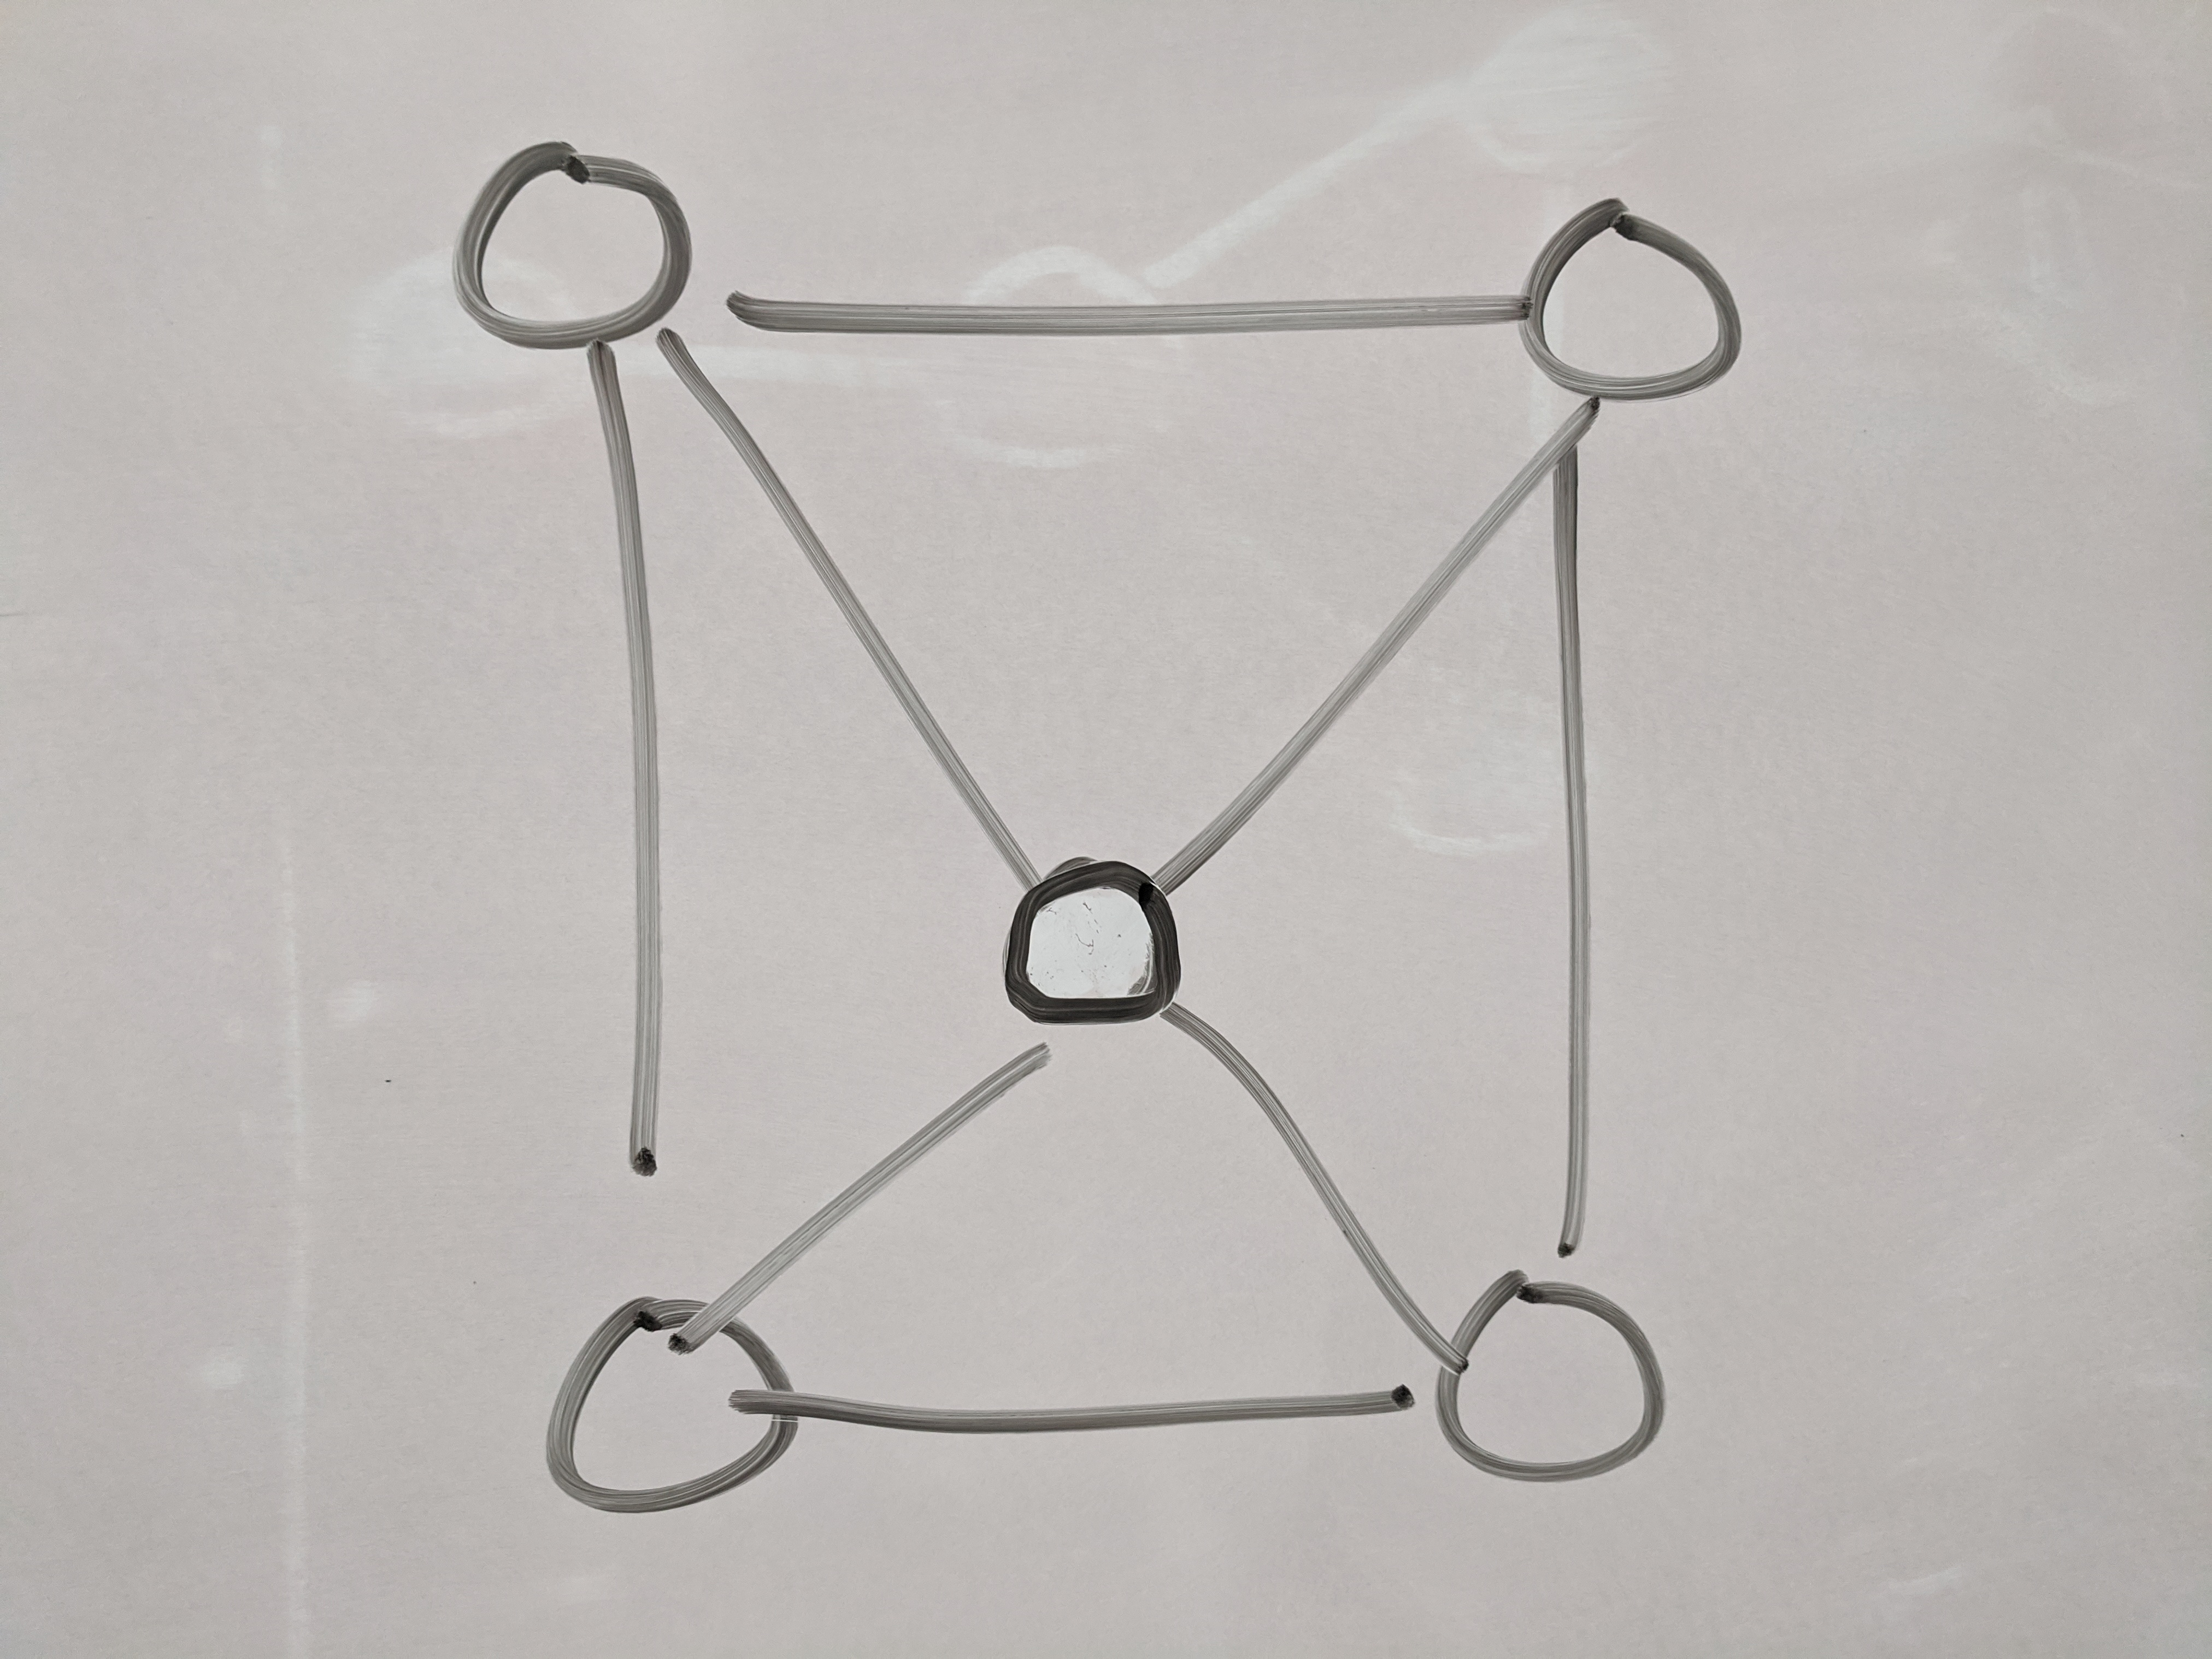
\includegraphics[height=100pt]{13-graph-uncolored.jpg}
    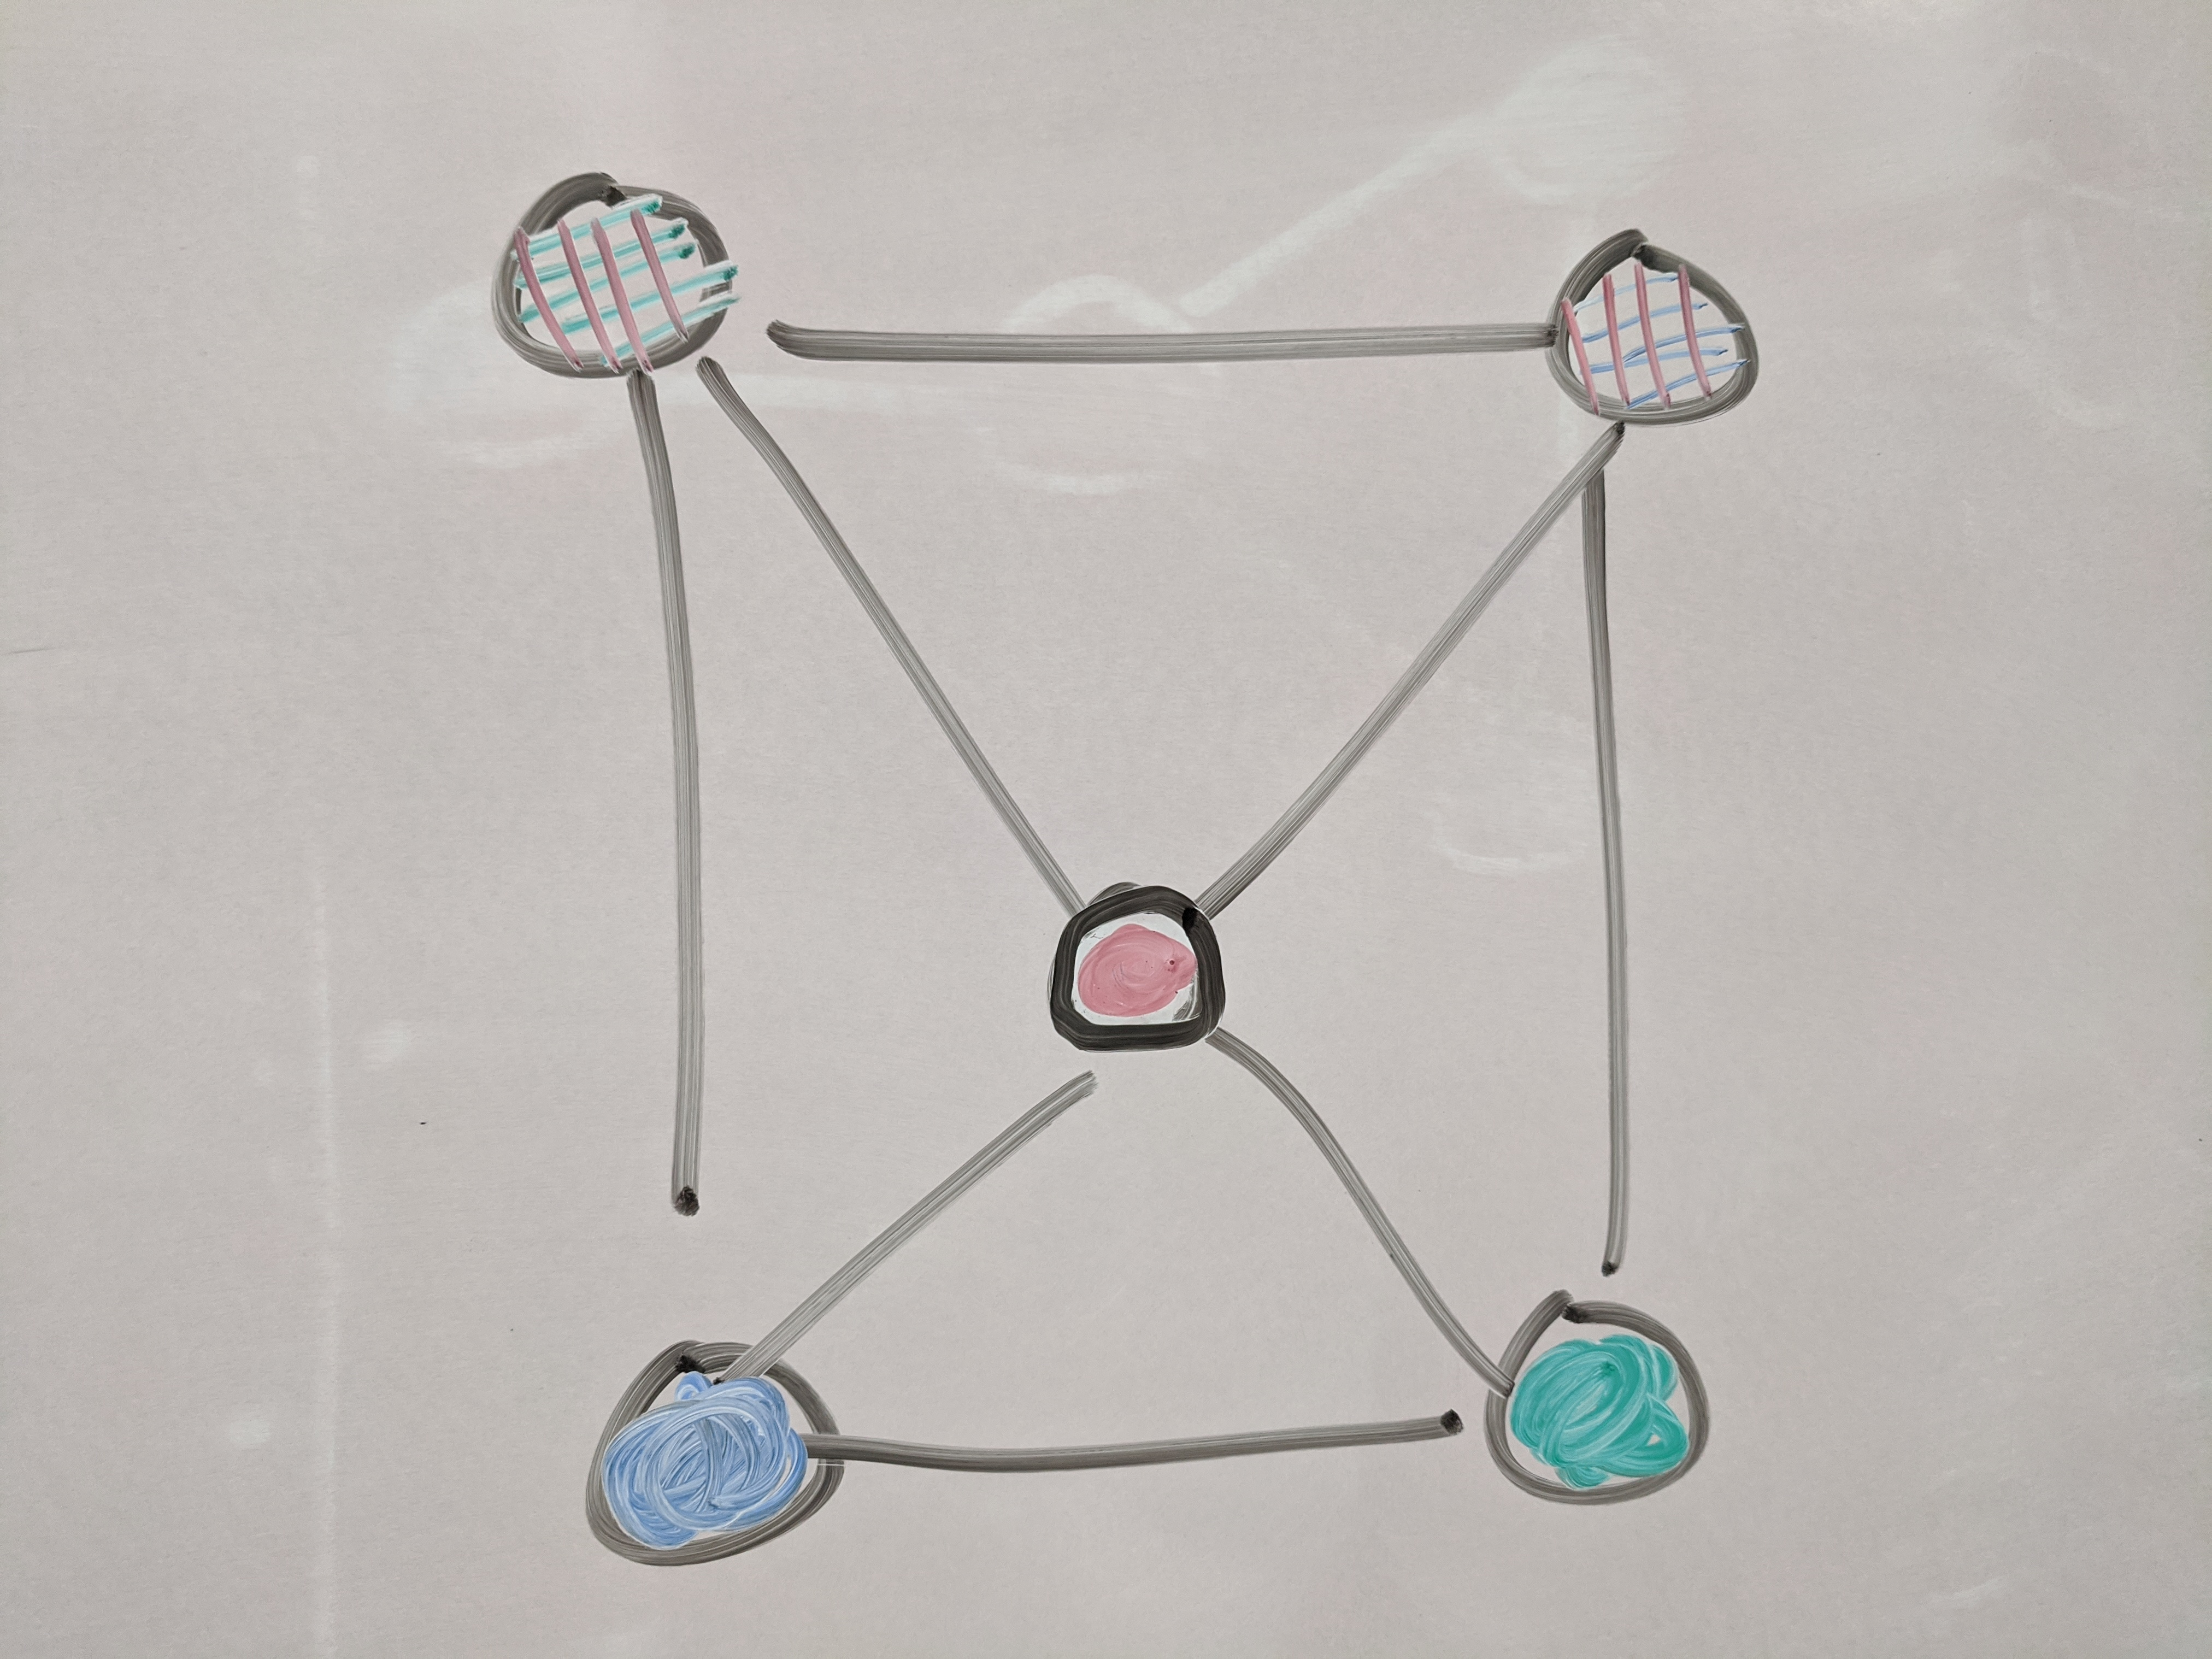
\includegraphics[height=100pt]{13-graph-colored-suboptimal.jpg}
    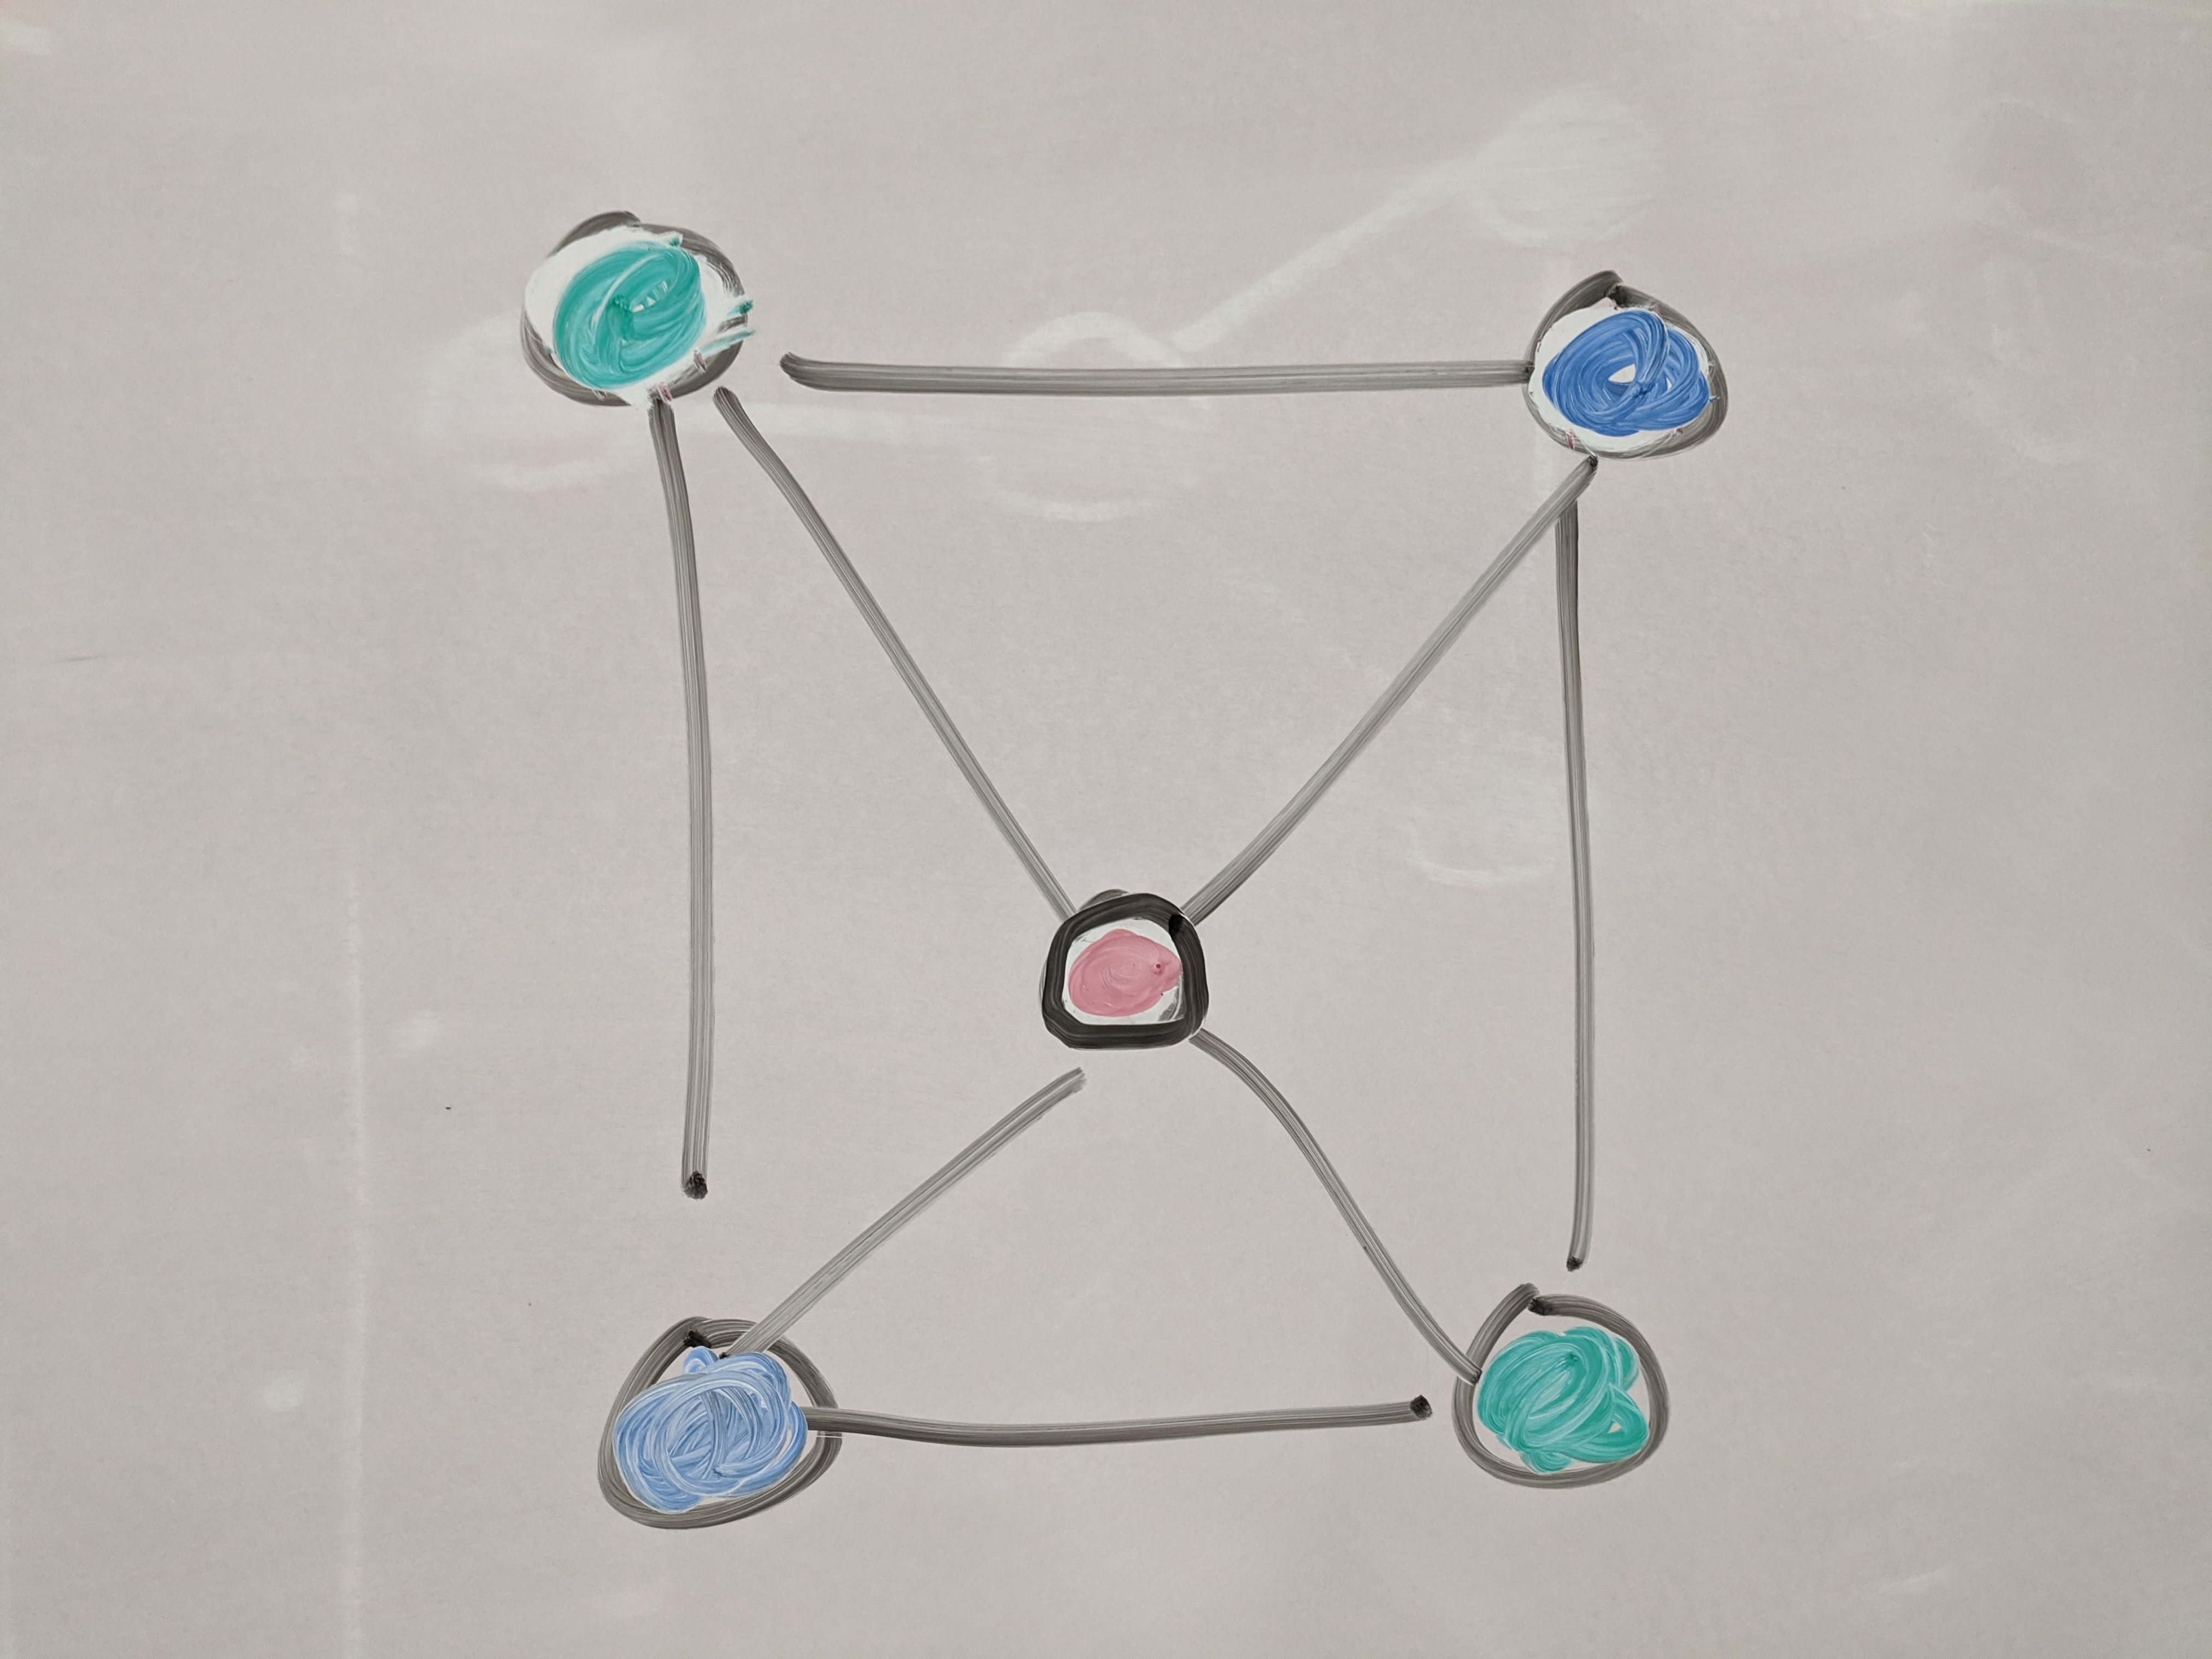
\includegraphics[height=100pt]{13-graph-colored-optimal.jpg}
  \end{center}
\end{frame}

\begin{frame} \frametitle{Approximation vs. Other Renegotiation Approaches}
Other ways of dealing with hard problems:
\begin{itemize}
  \item say ``no''
  \item when $n$ is tiny, settle for exponential-time algorithm
  \item no \emph{proof} of solution quality, but sometimes good enough:
    \begin{itemize}
      \item machine learning algorithms (also, humans don't need to precisely define what counts as ``correct'')
      \item heuristic algorithms
      \item Monte Carlo algorithms
    \end{itemize}
\end{itemize}

Approximation
\begin{itemize}
  \item pros: \emph{provable} solution quality, often fast
  \item con: relatively difficult alg. design and analysis
\end{itemize}
\end{frame}

\begin{frame} \frametitle{Performance Ratios}
\textbf{Approximation ratio} $\rho(n)$: ratio between quality of algorithm's output
and optimal output \stanza
\begin{itemize}
  \item smaller ratio is better
  \item 1 is perfect
  \item $\rho$ is defined differently for minimization, maximization problems
\end{itemize}
\end{frame}

\begin{frame} \frametitle{Performance Ratio for Minimization Problem}
  For \textbf{minimization} problem: if optimal quality is $C^\star$ and alg. produces
      quality $C,$ by definition $C^\star \leq C$ and define
      \[ \rho(n) = \frac{C}{C^\star} \]
  
  Recall 3-approx. vertex cover: \# colors $\leq 3 k^\star$
  \end{frame}
  
  \begin{frame} \frametitle{Performance Ratio for Maximization Problem}
For \textbf{maximization} problem: if optimal quality is $C^\star$ and alg. produces
    quality $C,$ by definition $C^\star \geq C,$ and define
    \[ \rho(n) = \frac{C^\star}{C} \]
  
    (Reciprocal of previous definition.)
    \stanza
    
    Consider approximate matching.

  \end{frame}

%\begin{frame} \frametitle{Fixed Approximation Ratios}
%Some approxmation algorithms have a fixed approximation ratio that is
%``baked in'' to the design of the algorithm. \stanza
%
%Ex.: algorithm that solves 3-approx. vertex cover would have fixed $\rho(n)=3$
%\stanza
%
%In general, better (smaller) ratios require slower algorithms. \\
%(note 1-approximation algorithms produce optimal solutions.) \stanza
%
%Deriving a different quality-vs.-time trade-off requires designing an
%entirely different algorithm.
%\end{frame}
%
%\begin{frame} \frametitle{Approximation Schemes}
%\textbf{approximation scheme}: family of related algorithms, such that, for
%any parameter $\epsilon > 0,$ scheme defines a
%$(1+\epsilon)$-approximate algorithm
%\begin{itemize}
%  \item think of $\epsilon$ as a \textbf{const} variable
%  \item time-performance trade-off is fully tuneable at compile time
%  \item user defines $\epsilon$ appropriately for their use case, recompiles
%  \item technically, changing $\epsilon$ defines a distinct algorithm
%  \item hence ``scheme''
%\end{itemize}
%\end{frame}
%
%\begin{frame} \frametitle{PTAS}
%\textbf{Polynomial Time Approximation Scheme (PTAS)}: approx. scheme where runtime
%is polynomial in $n$; nothing said of relationship to $\epsilon$ \\
%\begin{itemize}
%  \item ex. $O(2^{1/\epsilon} n \log n)$ \stanza
%\end{itemize}
%
%\textbf{\underline{Fully} PTAS}: runtime is polynomial in $n$ \underline{and} $1/\epsilon$ \\
%\begin{itemize}
%  \item ex. $O((1/\epsilon)^2 n^3)$
%  \item preferable to non-fully-PTAS
%\end{itemize}
%\end{frame}

\begin{frame} \frametitle{Vertex Cover Problem}
\emph{vertex cover problem} \\
\textbf{input}: undirected graph $G=(V,E)$ \\
\textbf{output}: set of vertices $C \subseteq V$, of minimal size $|C|,$ such
  that every edge in $E$ is incident on at least one vertex in $C$
 \stanza

 \emph{2-approximate vertex cover problem} \\
 \textbf{input}: undirected graph $G=(V,E)$ \\
 \textbf{output}: set of vertices $C \subseteq V$, such
   that every edge in $E$ is incident on at least one vertex in $C$, and
   $|C| \leq 2 |C^\star|$ where $C^\star$ is a minimal vertex cover for $G$
  \stanza

See Wiki page: \url{https://en.wikipedia.org/wiki/Vertex_cover}
\end{frame}

\begin{frame} \frametitle{Vertex Cover Example}
  \begin{center}
    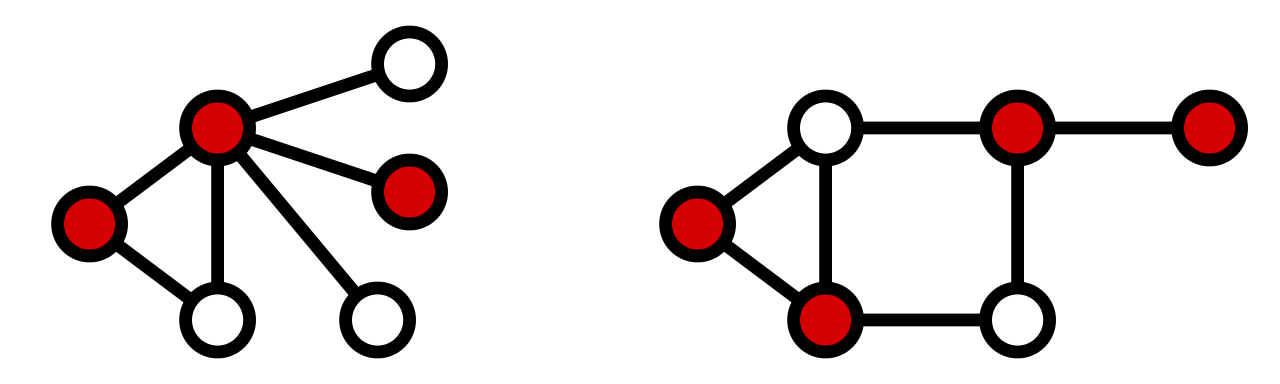
\includegraphics[height=80pt]{13-vertex-cover-1.png}
    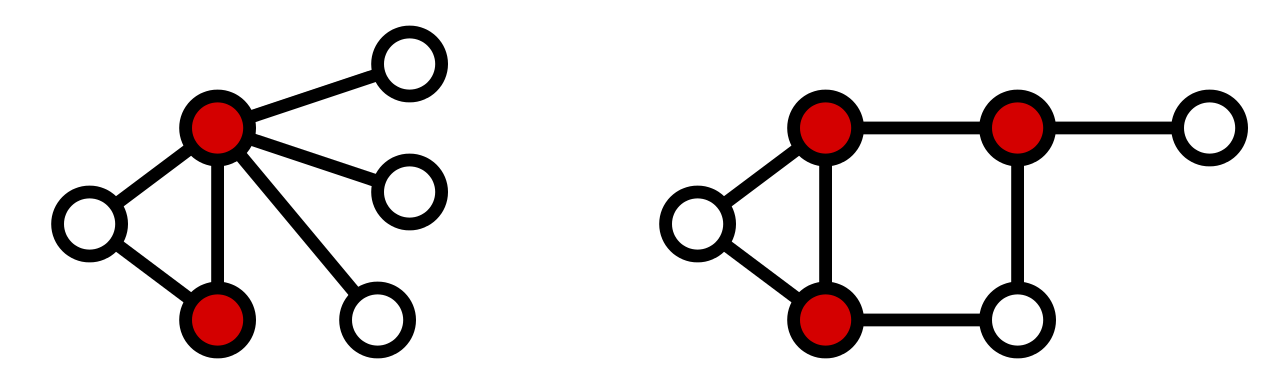
\includegraphics[height=80pt]{13-vertex-cover-2.png}
  \end{center}

  {\tiny
  Images credit: Wikipedia user Miym,
  \href{https://creativecommons.org/licenses/by-sa/3.0)}{CC BY-SA 3.0},
  \url{https://commons.wikimedia.org/wiki/File:Vertex-cover.svg},
  \url{https://commons.wikimedia.org/wiki/File:Minimum-vertex-cover.svg}
  }
\end{frame}

\begin{frame} \frametitle{Vertex Cover Hardness}
  \begin{itemize}
    \item vertex cover is $NP$-complete
    \item baseline algorithm:
    \begin{itemize}
      \item exhaustive search
      \item for each subset $C$ of vertices, check whether every edge has an
        endpoint in $C$
      \item return the smallest $C$ that is a valid cover
      \item $\Theta(2^n m)$ time, exponential, slow
    \end{itemize}
    \item goal of a 2-approximate vertex cover algorithm:
    \begin{itemize}
      \item get a decent (though imperfect) cover much faster
    \end{itemize}
  \end{itemize}
\end{frame}

\begin{frame} \frametitle{A Greedy Approximation Algorithm}
\begin{itemize}
  \item every edge $e=(u,v)$ needs both $u \in C$ and $v \in C$
  \item so grab an edge $e=(u,v)$ and include $u$ and $v$ in $C$
  \item every other edge touching $u$ or $v$ is now covered, so eliminate them
  \item continue until every edge is either grabbed or eliminated
\end{itemize}
\begin{center}
  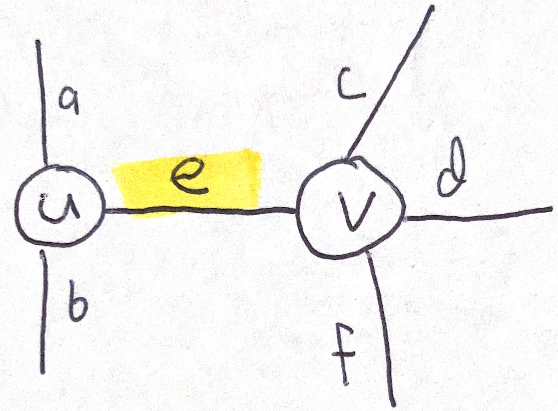
\includegraphics[height=100pt]{vertex-cover-greedy.png}
\end{center}
\end{frame}

\begin{frame} \frametitle{A Greedy Approximation Algorithm}
\begin{itemize}
    \item good: definitely finds a correct cover $C$
    \item bad: depending on the order of the ``grabs'', heuristic can get tricked
    into picking sub-optimal vertices
\end{itemize}
\end{frame}

\begin{frame} \frametitle{Example: Greedy Can Be Suboptimal}
\begin{center}
  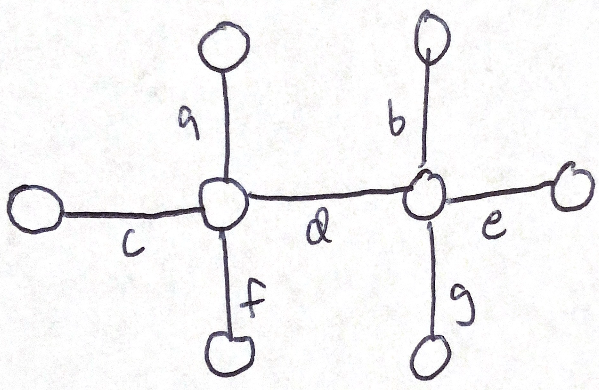
\includegraphics[height=100pt]{vertex-cover-counterexample.png}
  \stanza
  
  optimal edge choices: $d$ \stanza

  suboptimal edge choices: $a, b$ (and others)

\end{center}
\end{frame}
  
\begin{frame} \frametitle{2-Approximate Vertex Cover Pseudocode}
  \begin{algorithmic}[1]
    \Function{APPROX-VERTEX-COVER}{$G=(V,E)$}
      \State $C=\emptyset$
      \State $T=E$ \Comment{$T = $ edges that may be taken}
      \While { $T \ne \emptyset$ }
        \State Let $e=(u, v)$ be an arbitrary edge in $T$
        \State $C = C \cup \{u, v \}$
        \State Remove from $T$ any edge $f$ that is incident on $u$ or $v$
      \EndWhile
      \State \Return $C$
    \EndFunction
  \end{algorithmic}
\vspace{.5cm}
\textbf{Efficiency Analysis}: $O(m+n)$ time (assuming efficient data structures
for $G, T,$ and $C$)
\end{frame}

\begin{frame} \frametitle{Vertex Cover Performance Ratio}
\textbf{Lemma}: APPROX-VERTEX-COVER is a 2-approximation algorithm. \\
\textbf{Need:} for any $G, |C| \leq 2 |C^\star|$ \\
\textbf{Proof sketch}:
\begin{itemize}
  \item Let $A$ be the set of edges chosen inside the \textbf{while} loop
  \item will bound $|C|$ and $|C^\star|$ both in terms of $|A|$
\end{itemize}
\end{frame}
  
\begin{frame} \frametitle{Vertex Cover Performance Ratio (cont'd)}
\begin{itemize}
  \item \textbf{(1)} $|C^\star|$ vs. $|A|$
  \item $C^\star$ is a vertex cover, so for every edge $(u, v) \in A,$ we must have
    $u \in C^\star$ and/or $v \in C^\star$
  \item the ``Remove from $T$'' step guarantees that, after $(u, v)$ is chosen,
    no other edge incident on $u$ or $v$ will be chosen and added to $A$
  \item $\Rightarrow$ each vertex $x \in C^\star$ covers \emph{at most one} edge in $A$
  \item $\Rightarrow |C^\star| \geq |A|$
\end{itemize}
\end{frame}

\begin{frame} \frametitle{Vertex Cover Performance Ratio (cont'd)}
\begin{itemize}
  \item \textbf{(2)} $|C|$ vs. $|A|$
  \item the $C = C \cup \{u, v \}$ step inserts 2 vertices into $C$
  \item  due to the same ``Remove from $T$'' logic, neither $u$ nor $v$ was already
    in $C$
  \item $\Rightarrow |C| = 2|A|$ (note exact equality)
  \item \textbf{combining (1) and (2)}
  \begin{align*}
    |C| &= 2|A| \\
    & \leq 2(|C^\star|)
  \end{align*}
  \item QED
\end{itemize}
\end{frame}

\begin{frame} \frametitle{Commentary on this Proof}
\begin{itemize}
  \item optimal set cover $C^\star$ is opaque
  \item us analysts cannot know which vertices will be in a $C^\star$
  \item the algorithm doesn't know what $C^\star$ is, either
  \item all we do know is that, due to the definition of vertex cover, and
    the logic of our algorithm,
    \begin{center}
      \# vertices in optimal cover $\geq$ \# iterations \textbf{while} loop
    \end{center}
  \item and, due to algorithm logic,
  \begin{center}
      \# iterations \textbf{while} loop $=$ \# vertices chosen for approx. cover
  \end{center}
  \item in general, to prove an approx. ratio, need
  \begin{enumerate}
    \item to bound quality of arbitrary, opaque optimal solution; and
    \item bound quality of approx. solution the same way
  \end{enumerate}
\end{itemize}
\end{frame}

\begin{frame} \frametitle{TSP}
  \emph{traveling salesperson problem (TSP)} \\
  \textbf{input}: a complete undirected graph $G=(V,E)$ where each edge has weight $w(e) \geq 0$ \\
  \textbf{output}: a sequence of vertices $H$ forming a Hamiltonian cycle, minimizing
  total edge weight
  \stanza
  
  Recall:
  \begin{itemize}
    \item \emph{Cycle:} path that starts and ends at same vertex
    \item \emph{Hamiltonian:} visits each vertex exactly once
    \item every complete graph contains some Hamiltonian cycle
  \end{itemize}
  
  \textbf{Bad news:}
  \begin{itemize}
    \item TSP is $NP$-complete; if $P \ne NP$, no polynomial-time optimization algorithm
    \item TSP is also $APX$-complete; if $P \ne NP,$ no PTAS
  \end{itemize}
  \end{frame}
  
  \begin{frame} \frametitle{TSP}
    \begin{center}
      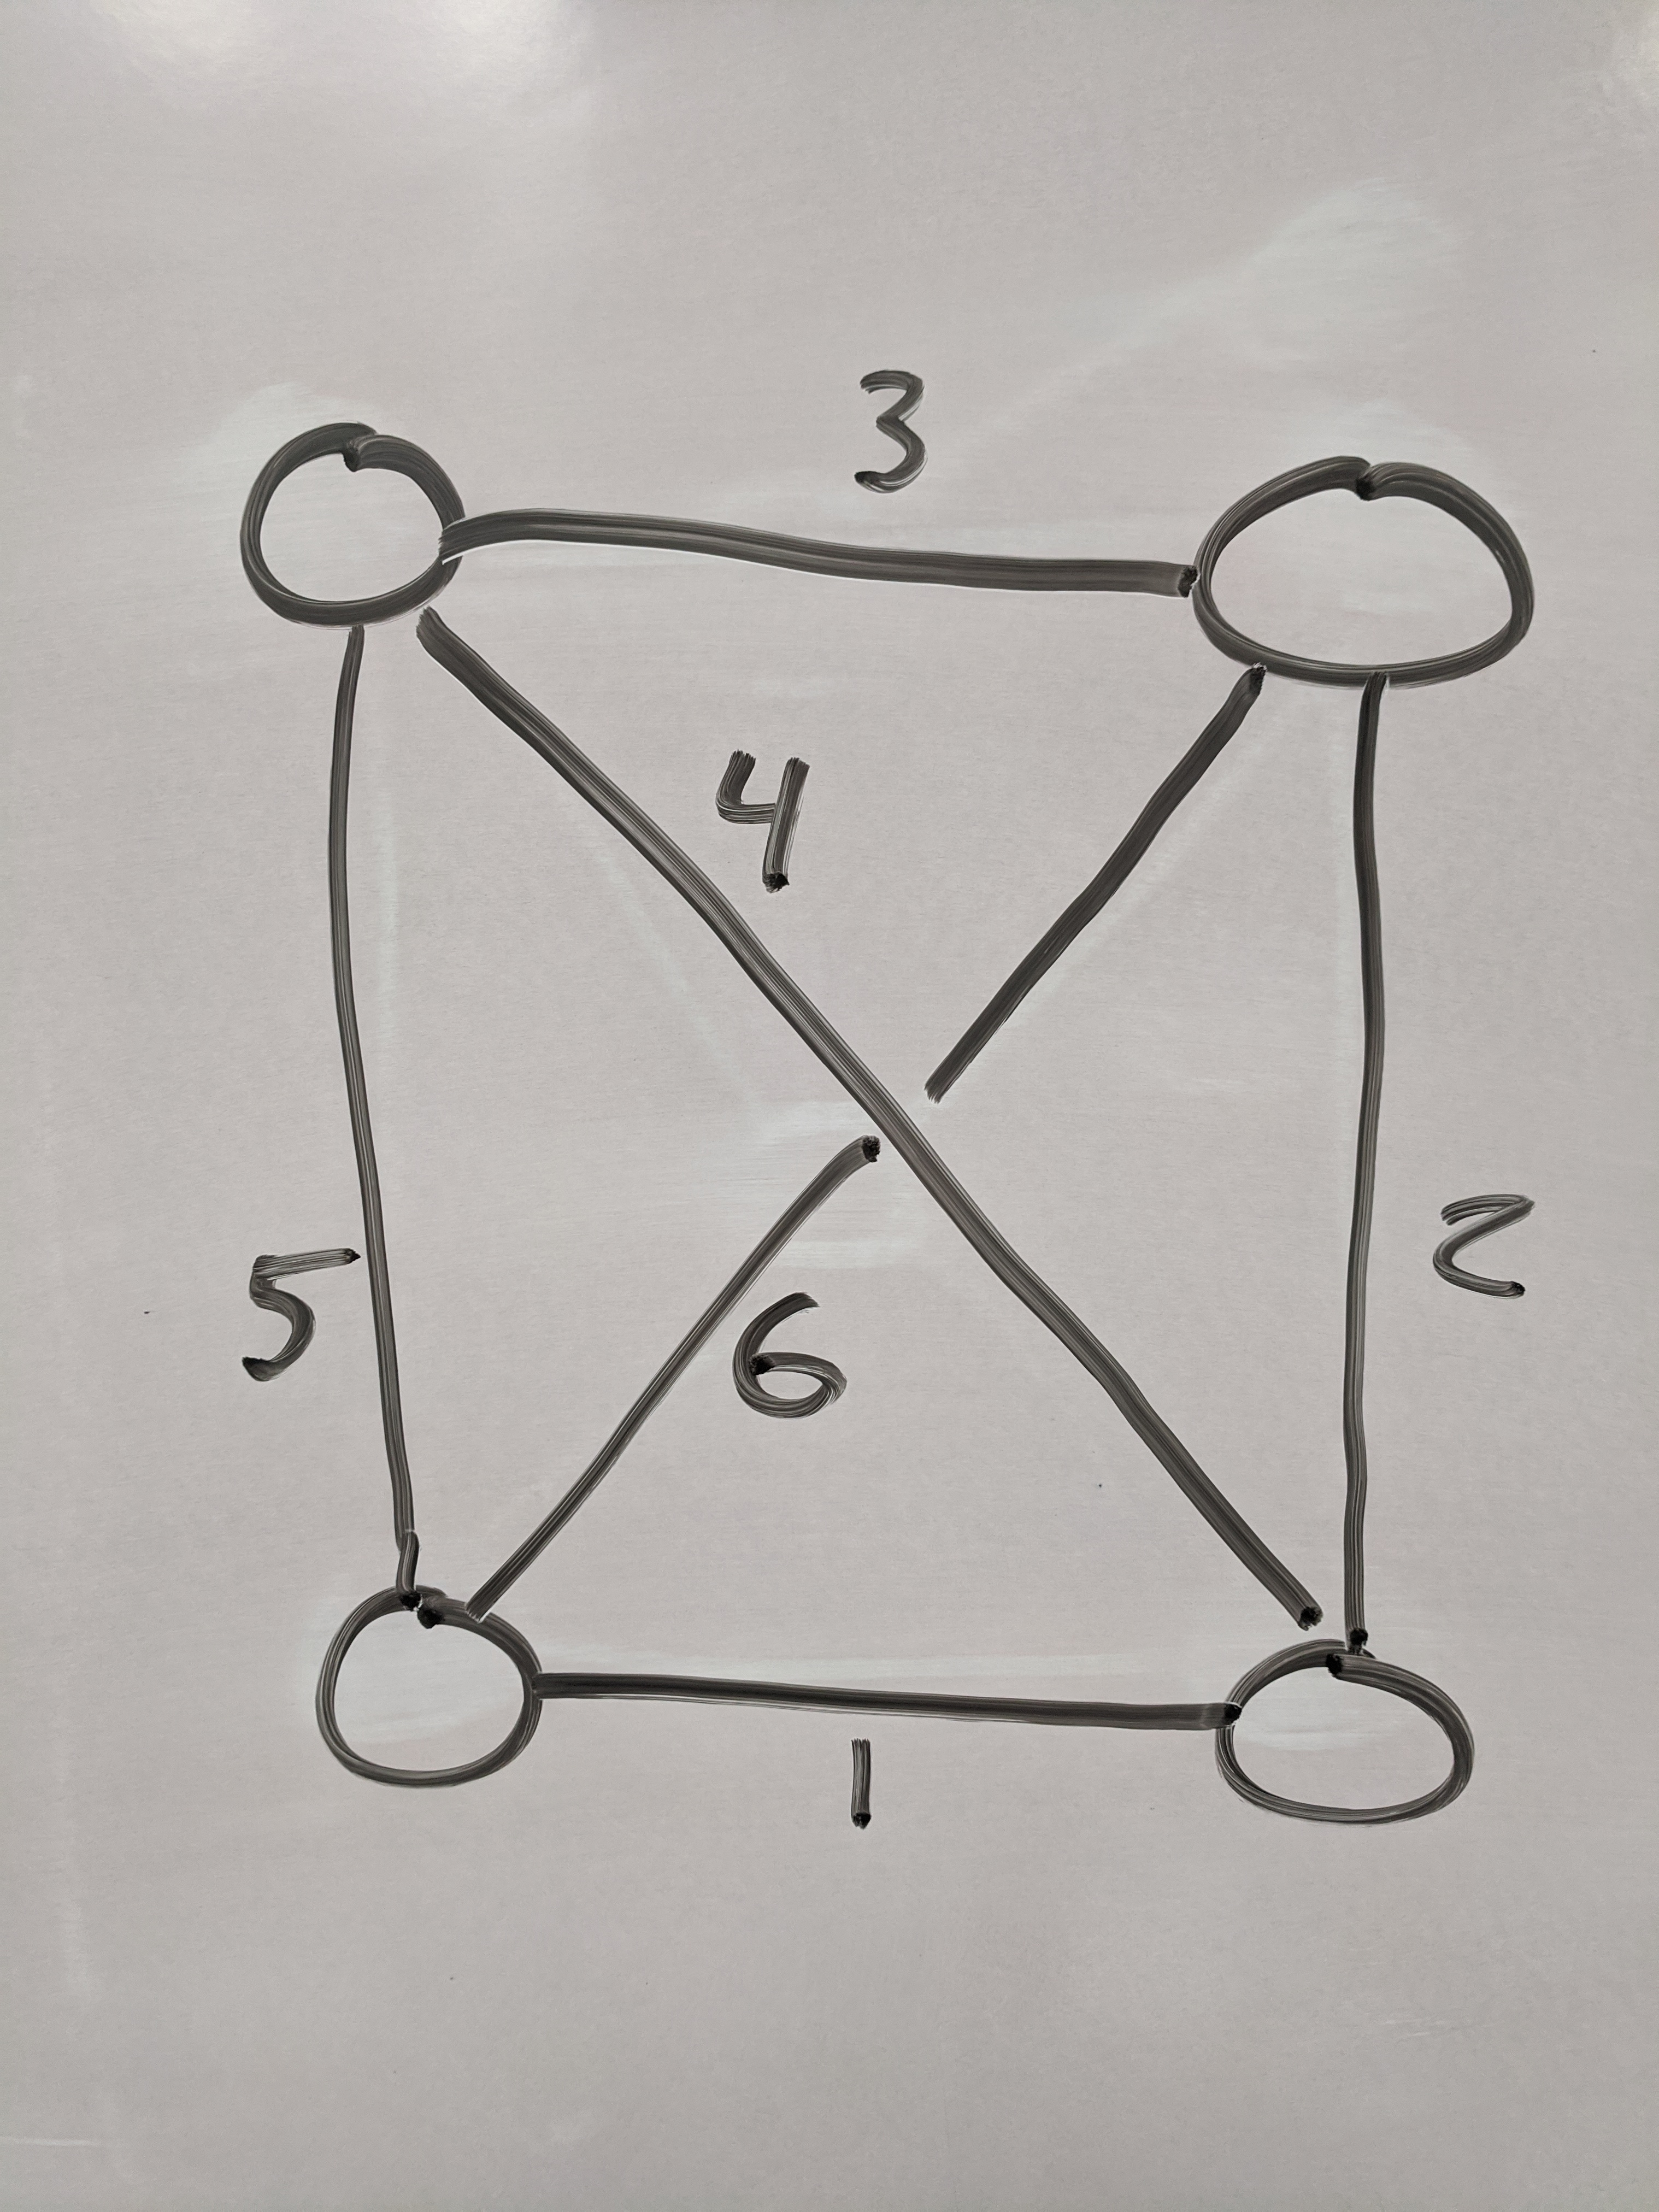
\includegraphics[height=120pt]{13-tsp-input.jpg}
      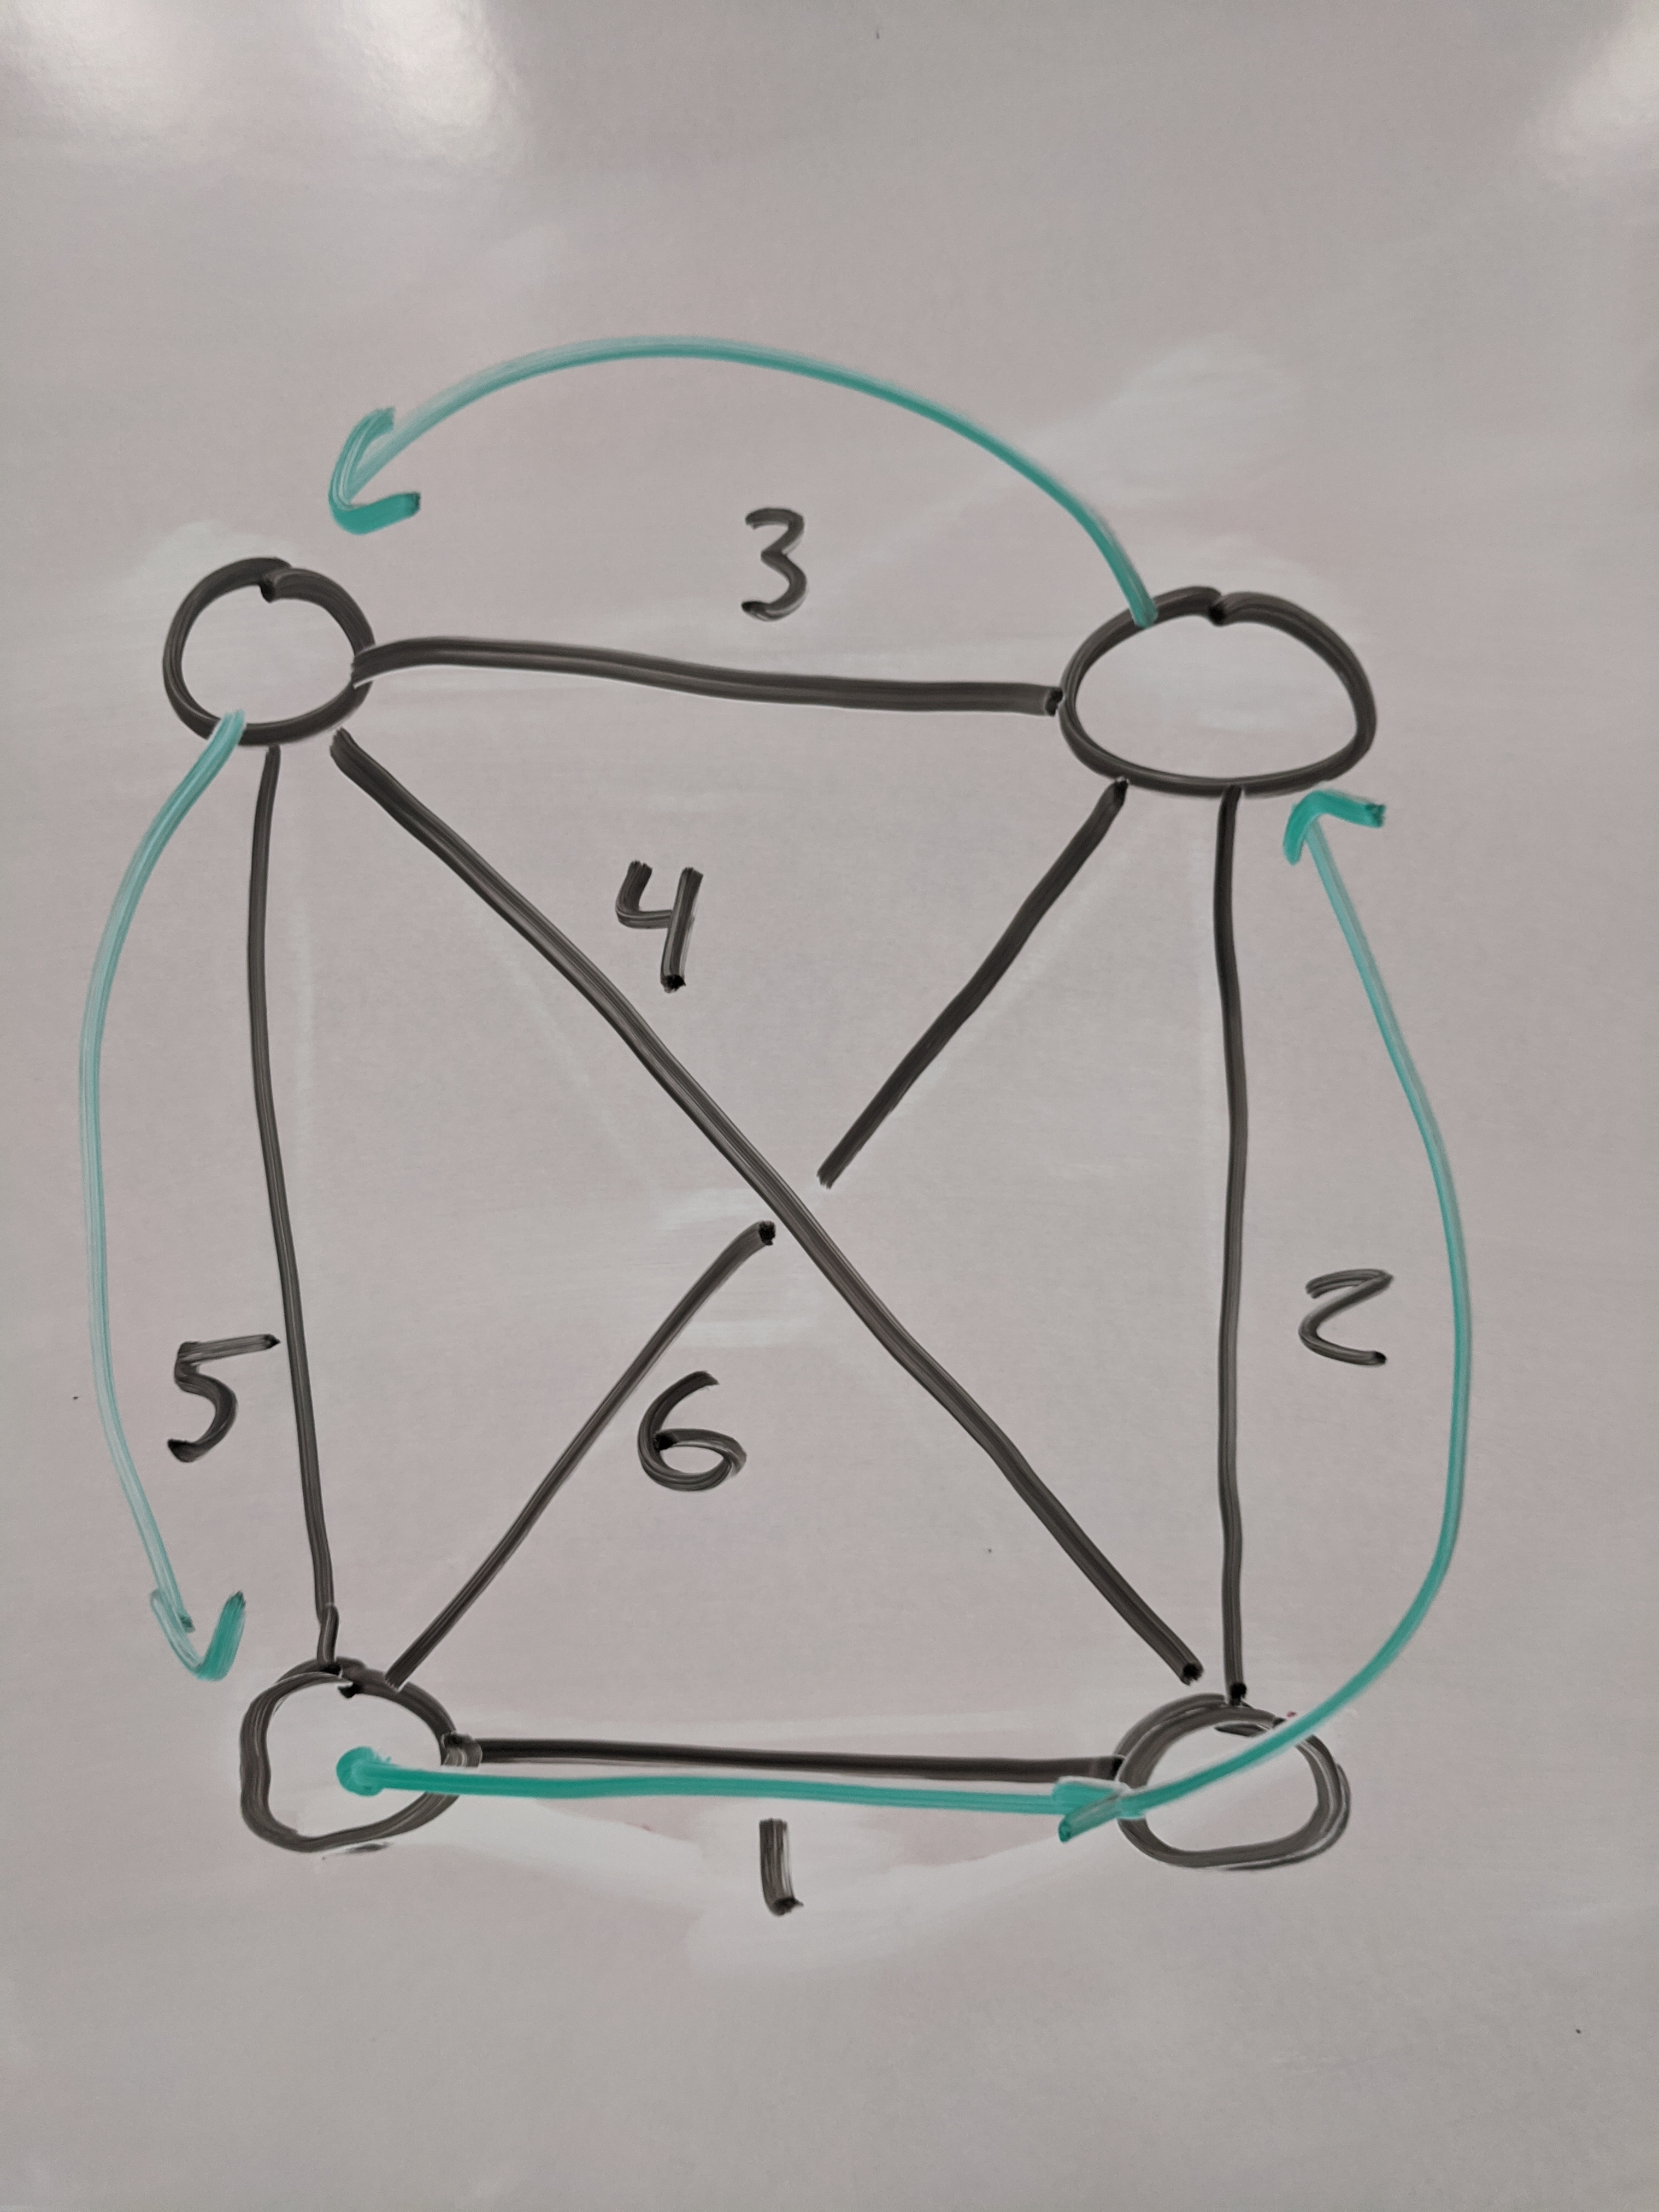
\includegraphics[height=120pt]{13-tsp-output.jpg}
    \end{center}
  \end{frame}
  
  \begin{frame} \frametitle{Triangle Inequality}
  Triangle inequality in general: for distance function $d$ and sites $a, b, c,$
  \[ d(a, c) \leq d(a, b) + d(b, c) \]
  $\Rightarrow$ direct path $a \rightarrow c$ always cheaper than two-step path
  $a \rightarrow b \rightarrow c$ (or tied) \stanza
  
  Triangle inequality in a complete graph: for vertices $x, y, z$ and edge weights $w,$
  \[ w(x, z) \leq w(x, y) + w(y, z) \]
  $\Rightarrow$ same intuition; adding an intermediate step is never a shortcut \\
  $\Rightarrow$ automatically holds for Euclidean graphs
  \end{frame}
  
  \begin{frame} \frametitle{TSP with Triangle Inequality (TSPTI)}
  
  \textbf{input}: a complete undirected graph $G=(V,E)$ where each edge has weight $w(e) \geq 0$;
  and for any $x, y, z \in V$, $w(x, z) \leq w(x, y) + w(y, z)$ \\
  \textbf{output}: (same as conventional TSP) \stanza
  \begin{itemize}
    \item \textbf{renegotiating} TSP
    \item different problem; $NP$-completeness and $APX$-completeness proofs may not apply
    \item less-general problem
    \item probably still relevant to practical applications of TSP
  \end{itemize}
  \end{frame}
  
  \begin{frame} \frametitle{TSPTI Approximation Algorithm Idea}
  \begin{itemize}
    \item need a structure that can lower-bound an optimal cycle $H^\star$ and upper-bound
      our approximate cycle $H$
    \item \emph{minimum spanning tree} features
    \begin{itemize}
      \item minimizes weight of chosen edges
      \item connects all vertices
      \item can be computed fast
    \end{itemize}
    \item but an MST is not a Hamiltonian cycle; MST is acyclic, for one thing
    \item \emph{Euler tour:} cycle around a tree; preorder, inorder, postorder
    \item build an MST; perform preorder traversal; treat that vertex order as Hamiltonian cycle
  \end{itemize}
  \end{frame}
  
  \begin{frame} \frametitle{Review: Minimum Spanning Trees (MST)}
    \begin{center}
      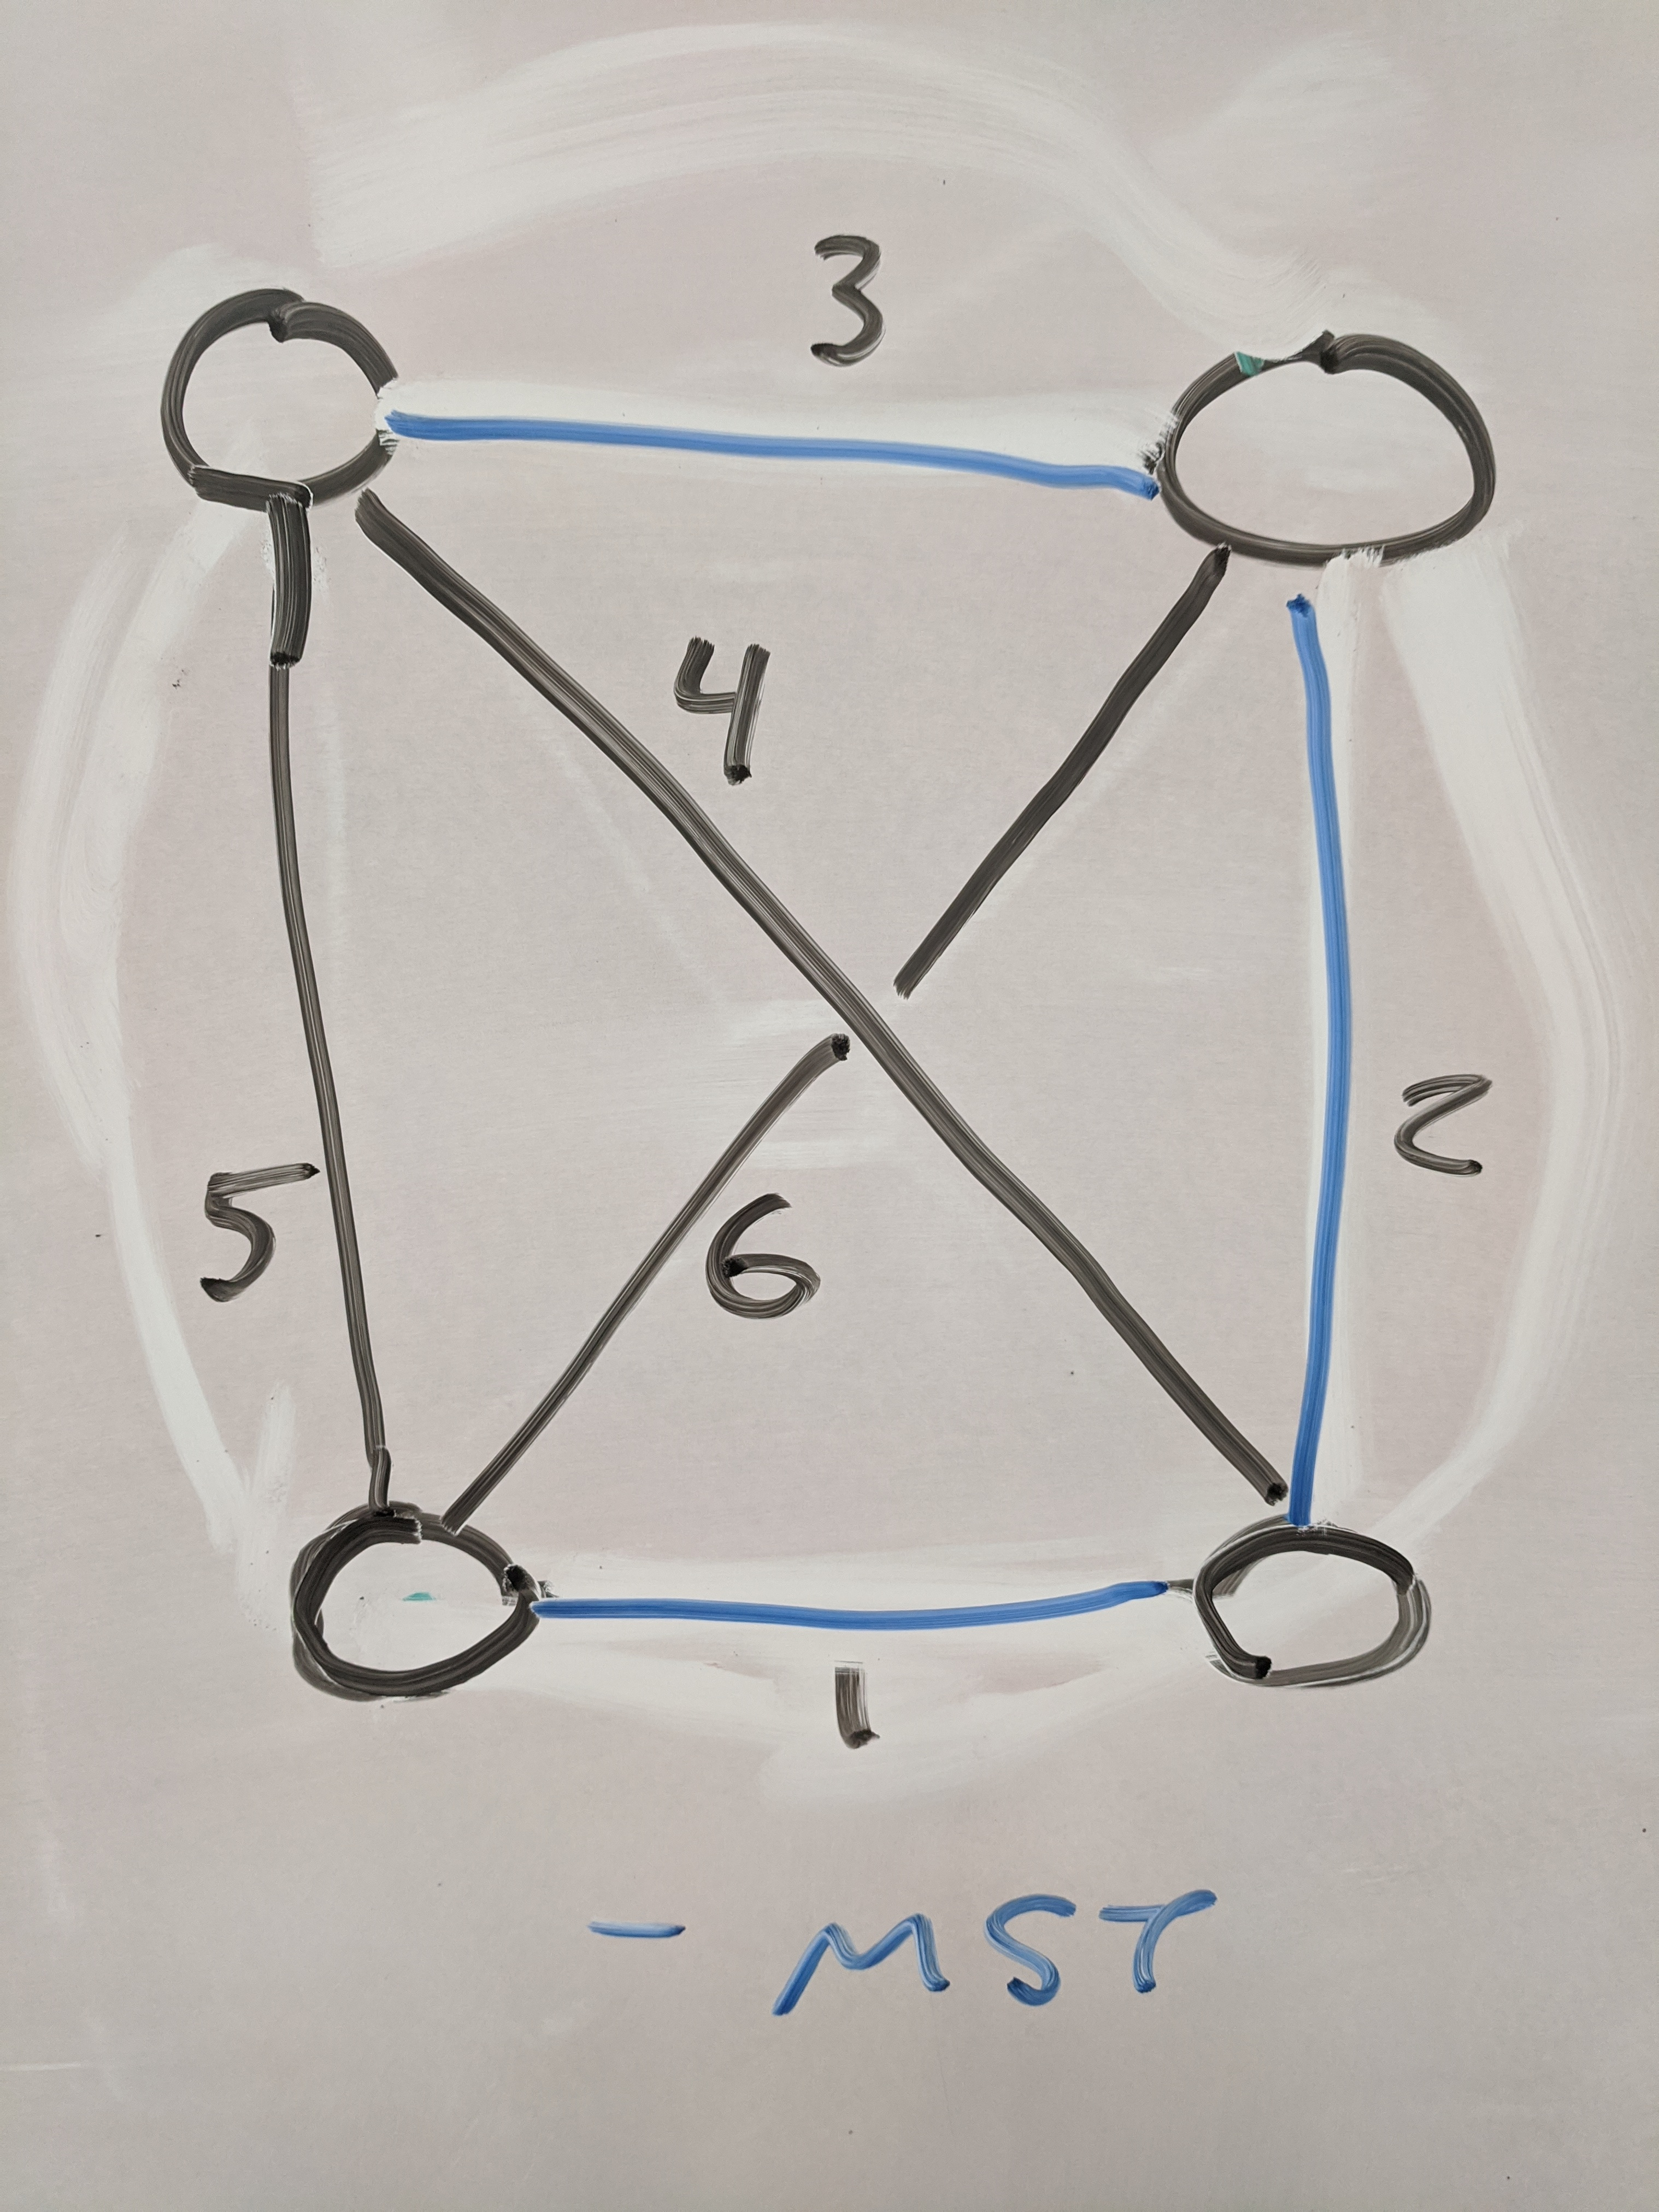
\includegraphics[height=160pt]{13-mst.jpg}
    \end{center}
  \end{frame}
  
  \begin{frame} \frametitle{Review: Preorder Traversal}
    \begin{center}
      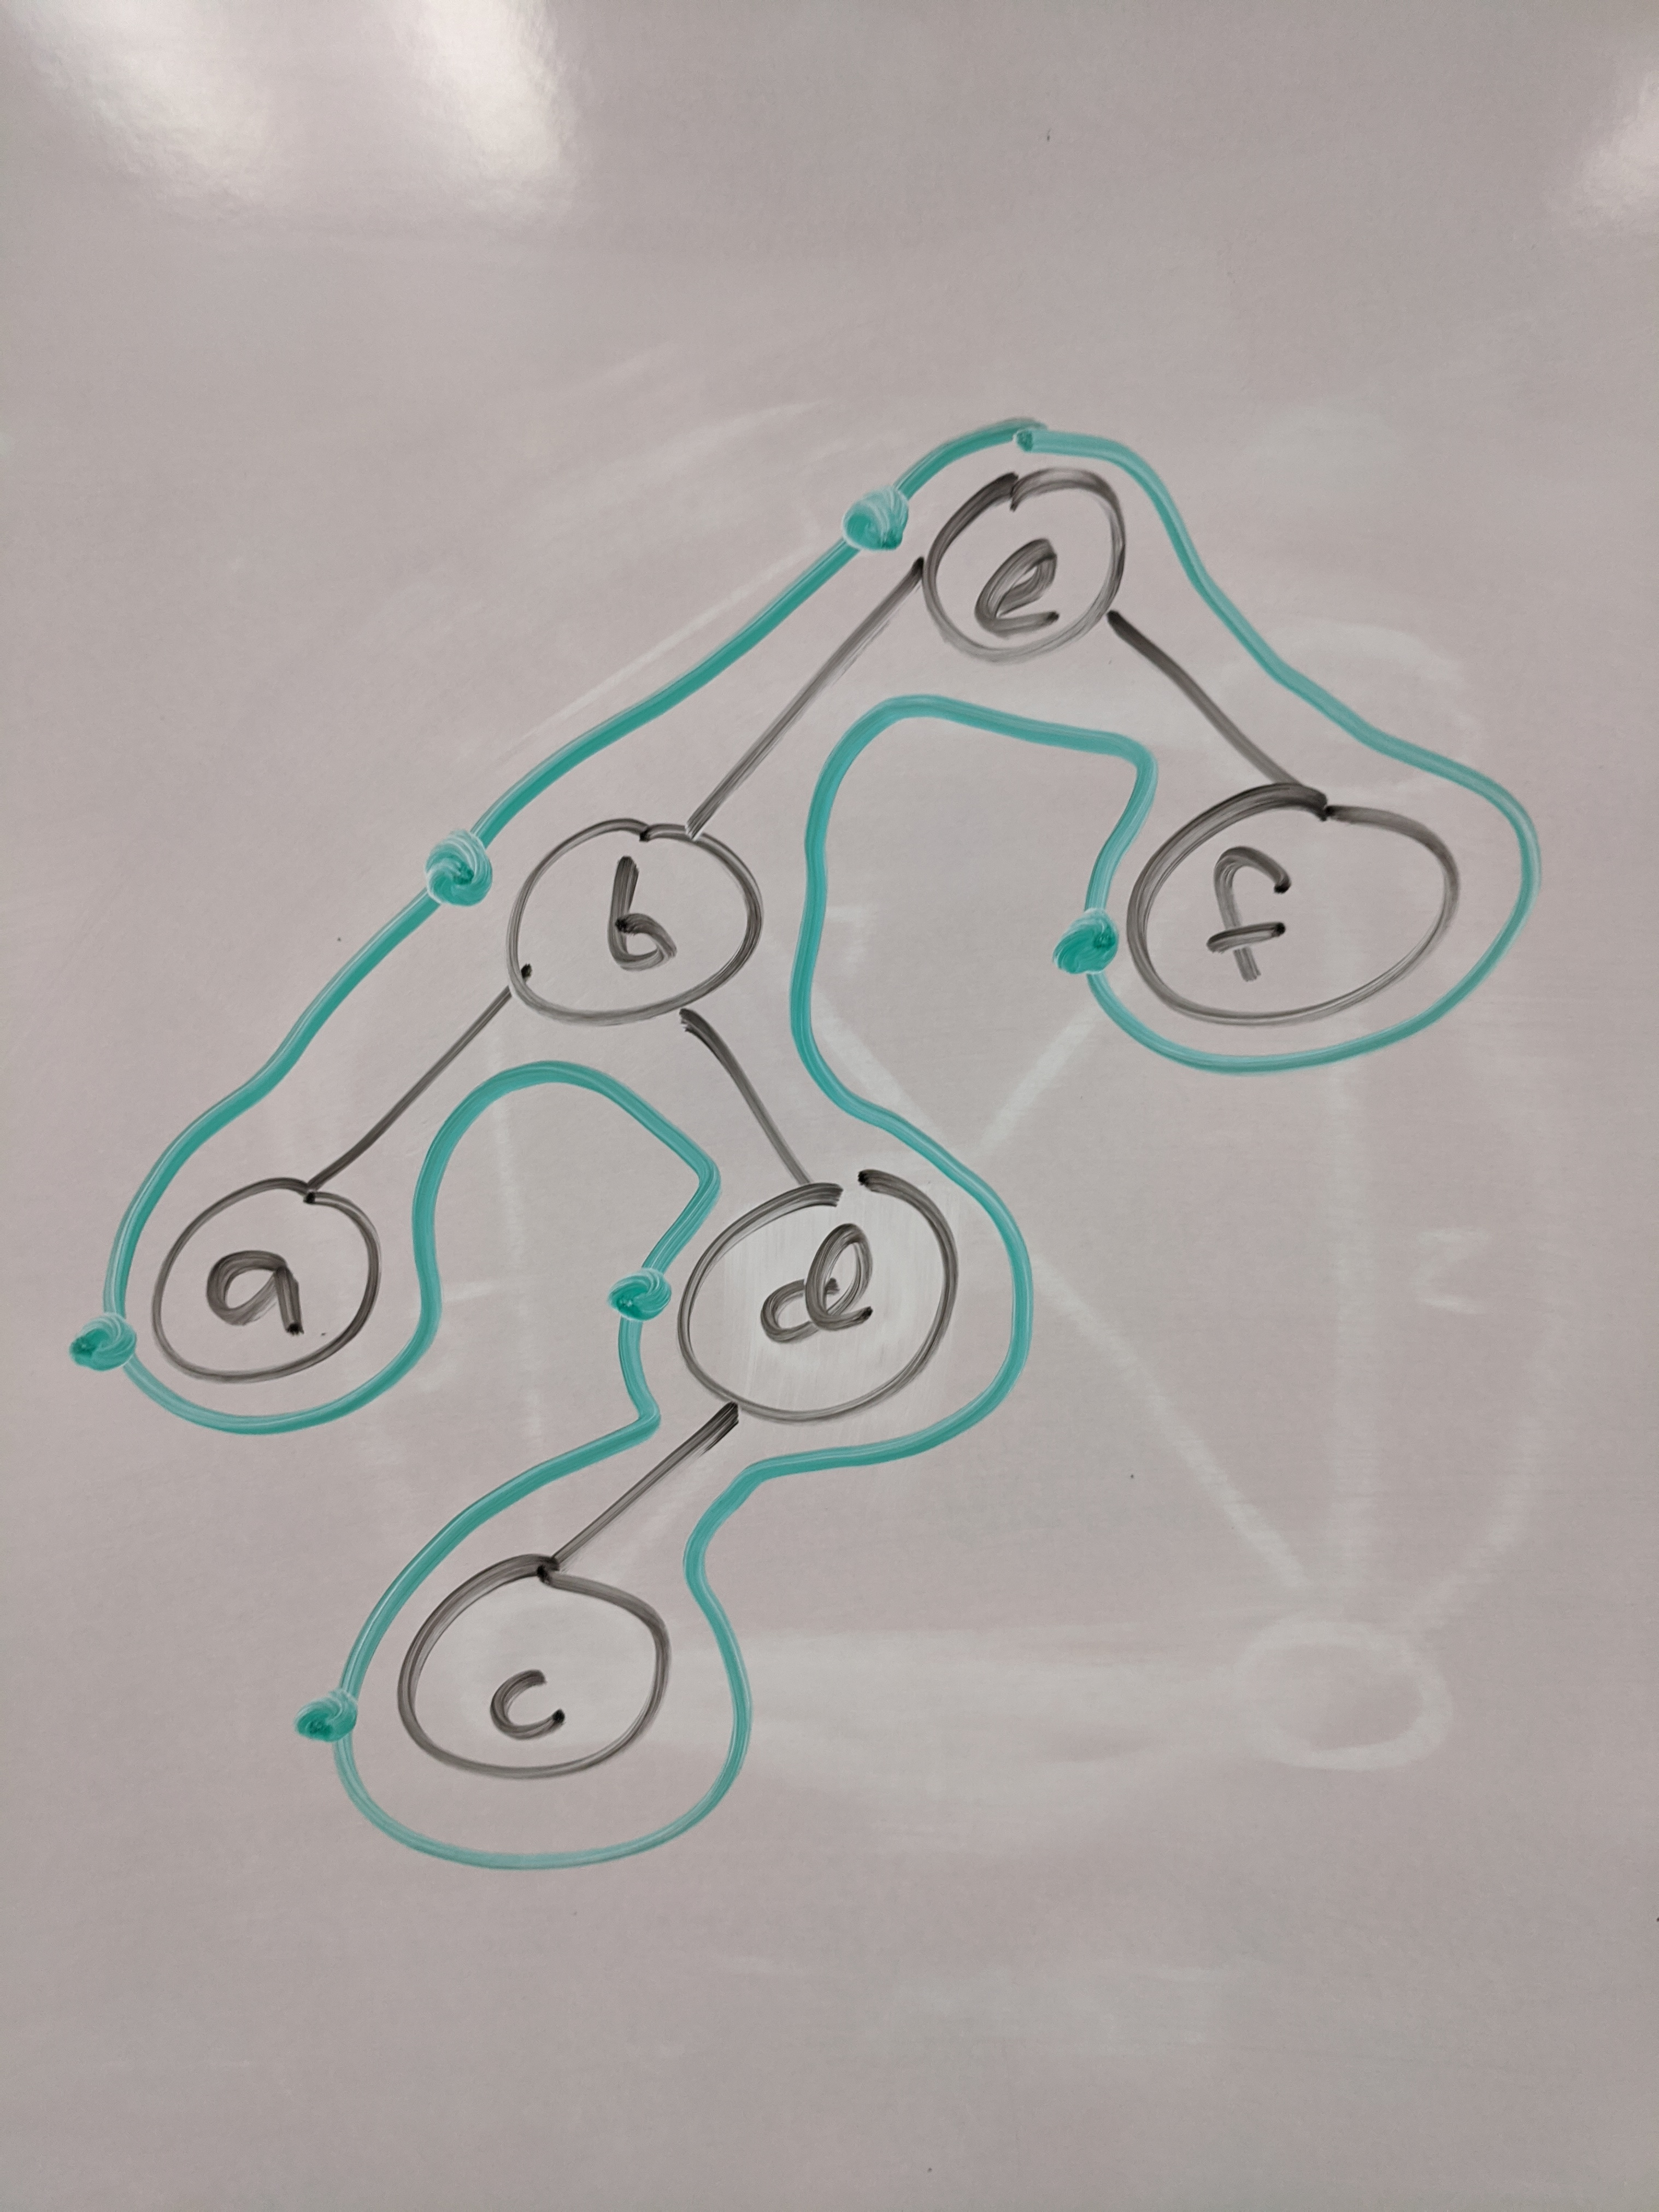
\includegraphics[height=160pt]{13-preorder.jpg}
    \end{center}
  \end{frame}
  
  \begin{frame} \frametitle{Approximate TSPTI Pseudocode}
    \begin{algorithmic}[1]
      \Function{APPROX-TSPTI}{$G=(V,E), w$}
        \State $T = PRIM-MST(G, w)$
        \State $H = $ empty sequence of vertices
        \For { vertex $v$ in preorder traversal of tree $T$ }
          \State $H.ADDBACK(v)$
        \EndFor
        \State $H.ADDBACK(H[0])$
        \State \Return $H$
      \EndFunction
    \end{algorithmic}
  \vspace{.5 cm}
  \textbf{Analysis}: Prim's algorithm takes $O(m + n \log n)$ (w/ Fibonacci heap),
  traversal takes $O(m + n)$, total $O(m + n \log n)$ time
  \end{frame}
  
  \begin{frame} \frametitle{Approximate TSPTI: MST}
    \begin{center}
      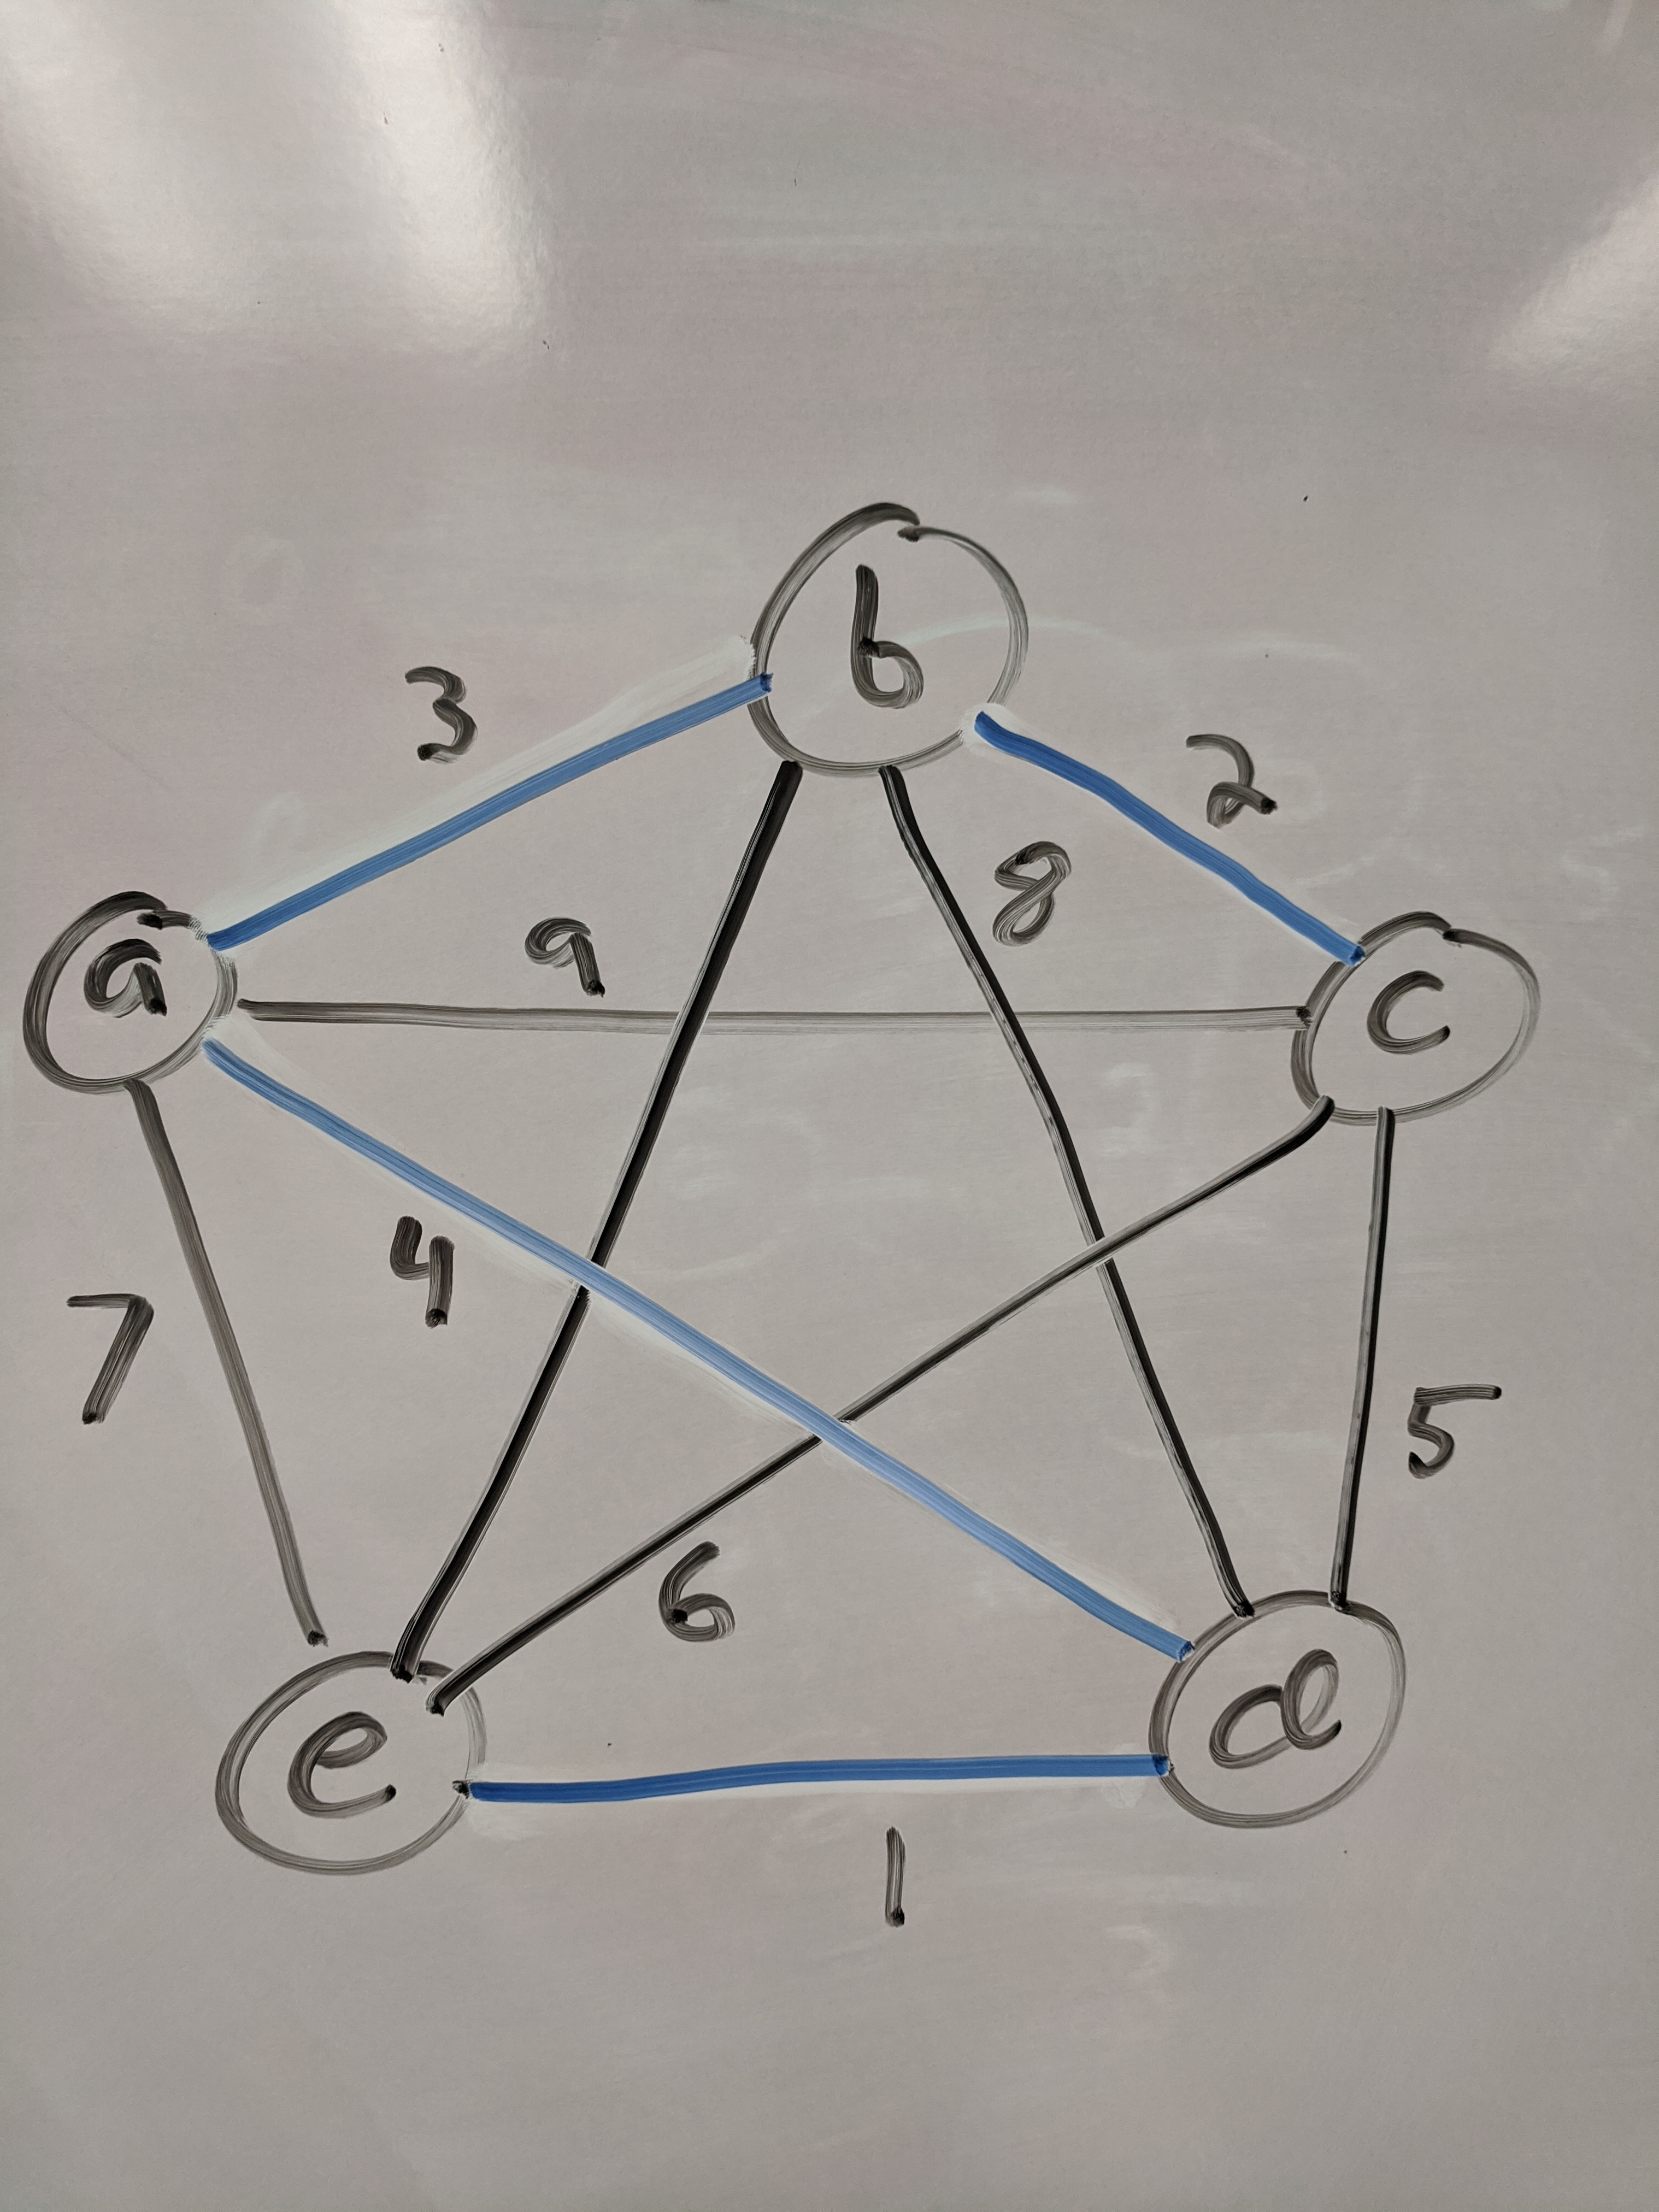
\includegraphics[height=160pt]{13-tspti-mst.jpg}
    \end{center}
  \end{frame}
  
  \begin{frame} \frametitle{Approximate TSPTI: Preorder Traversal}
    \begin{center}
      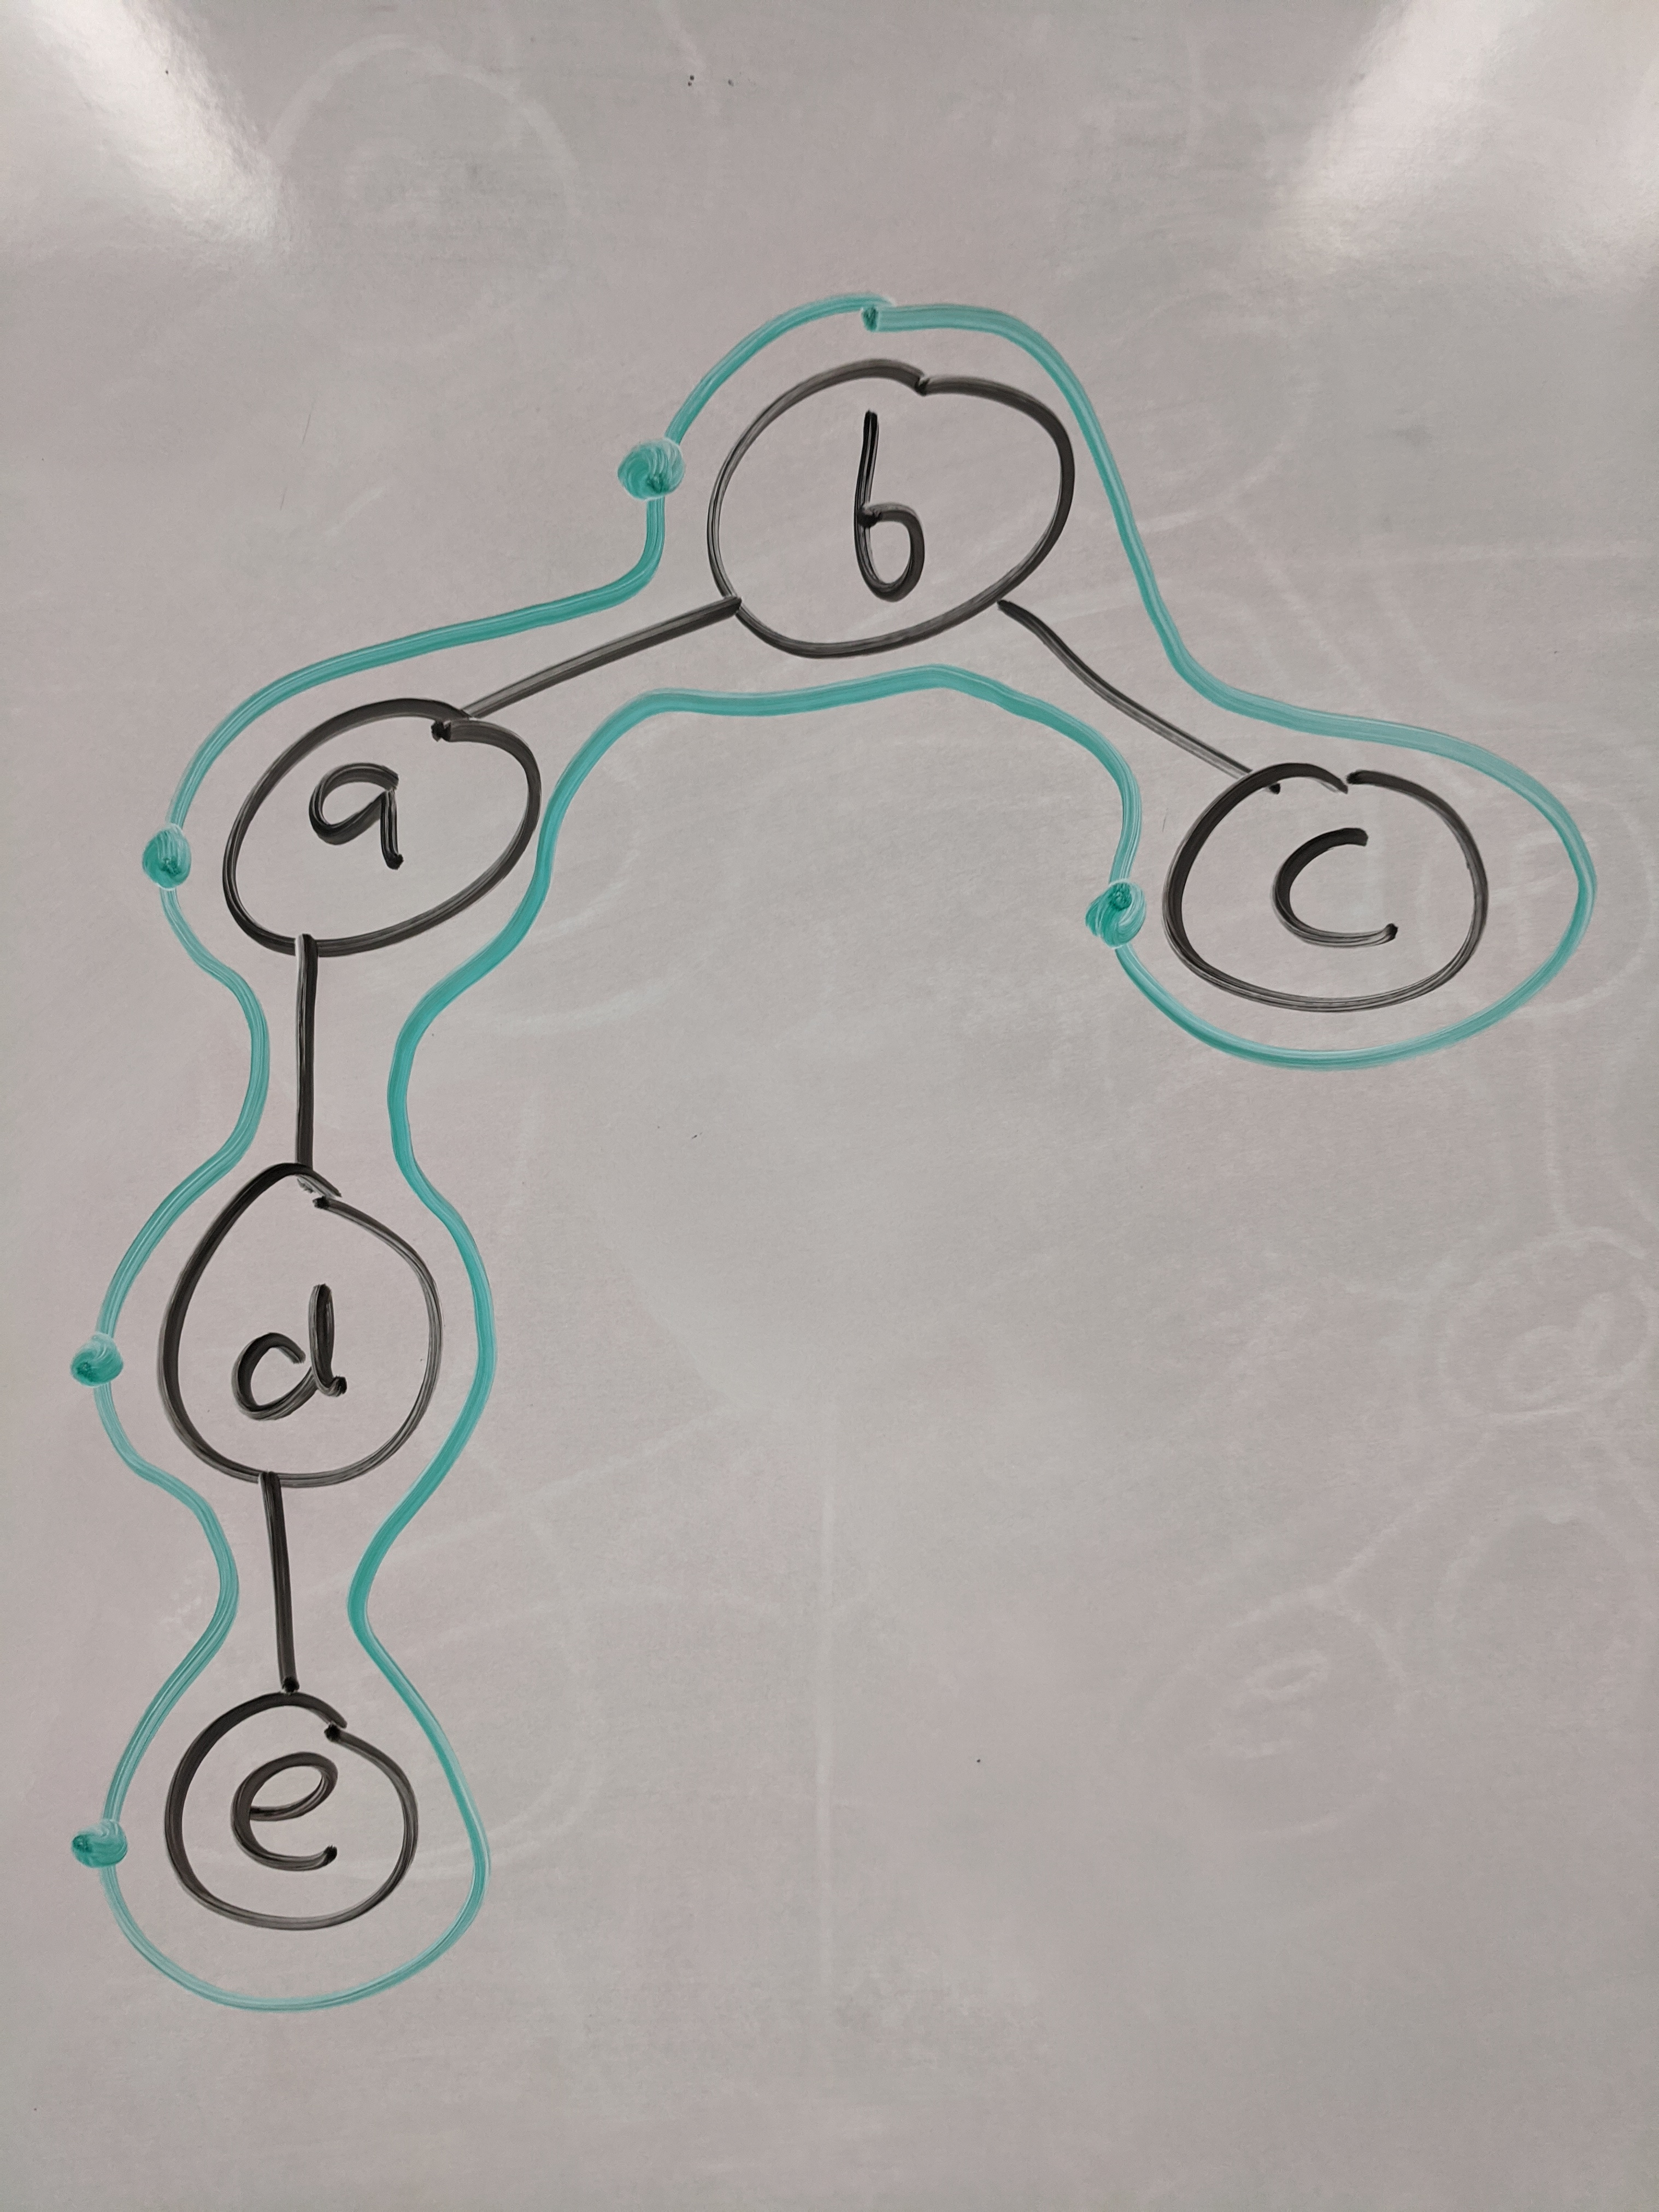
\includegraphics[height=160pt]{13-tspti-preorder.jpg}
    \end{center}
  \end{frame}
  
  \begin{frame} \frametitle{Approximate TSPTI: Solution}
    \begin{center}
      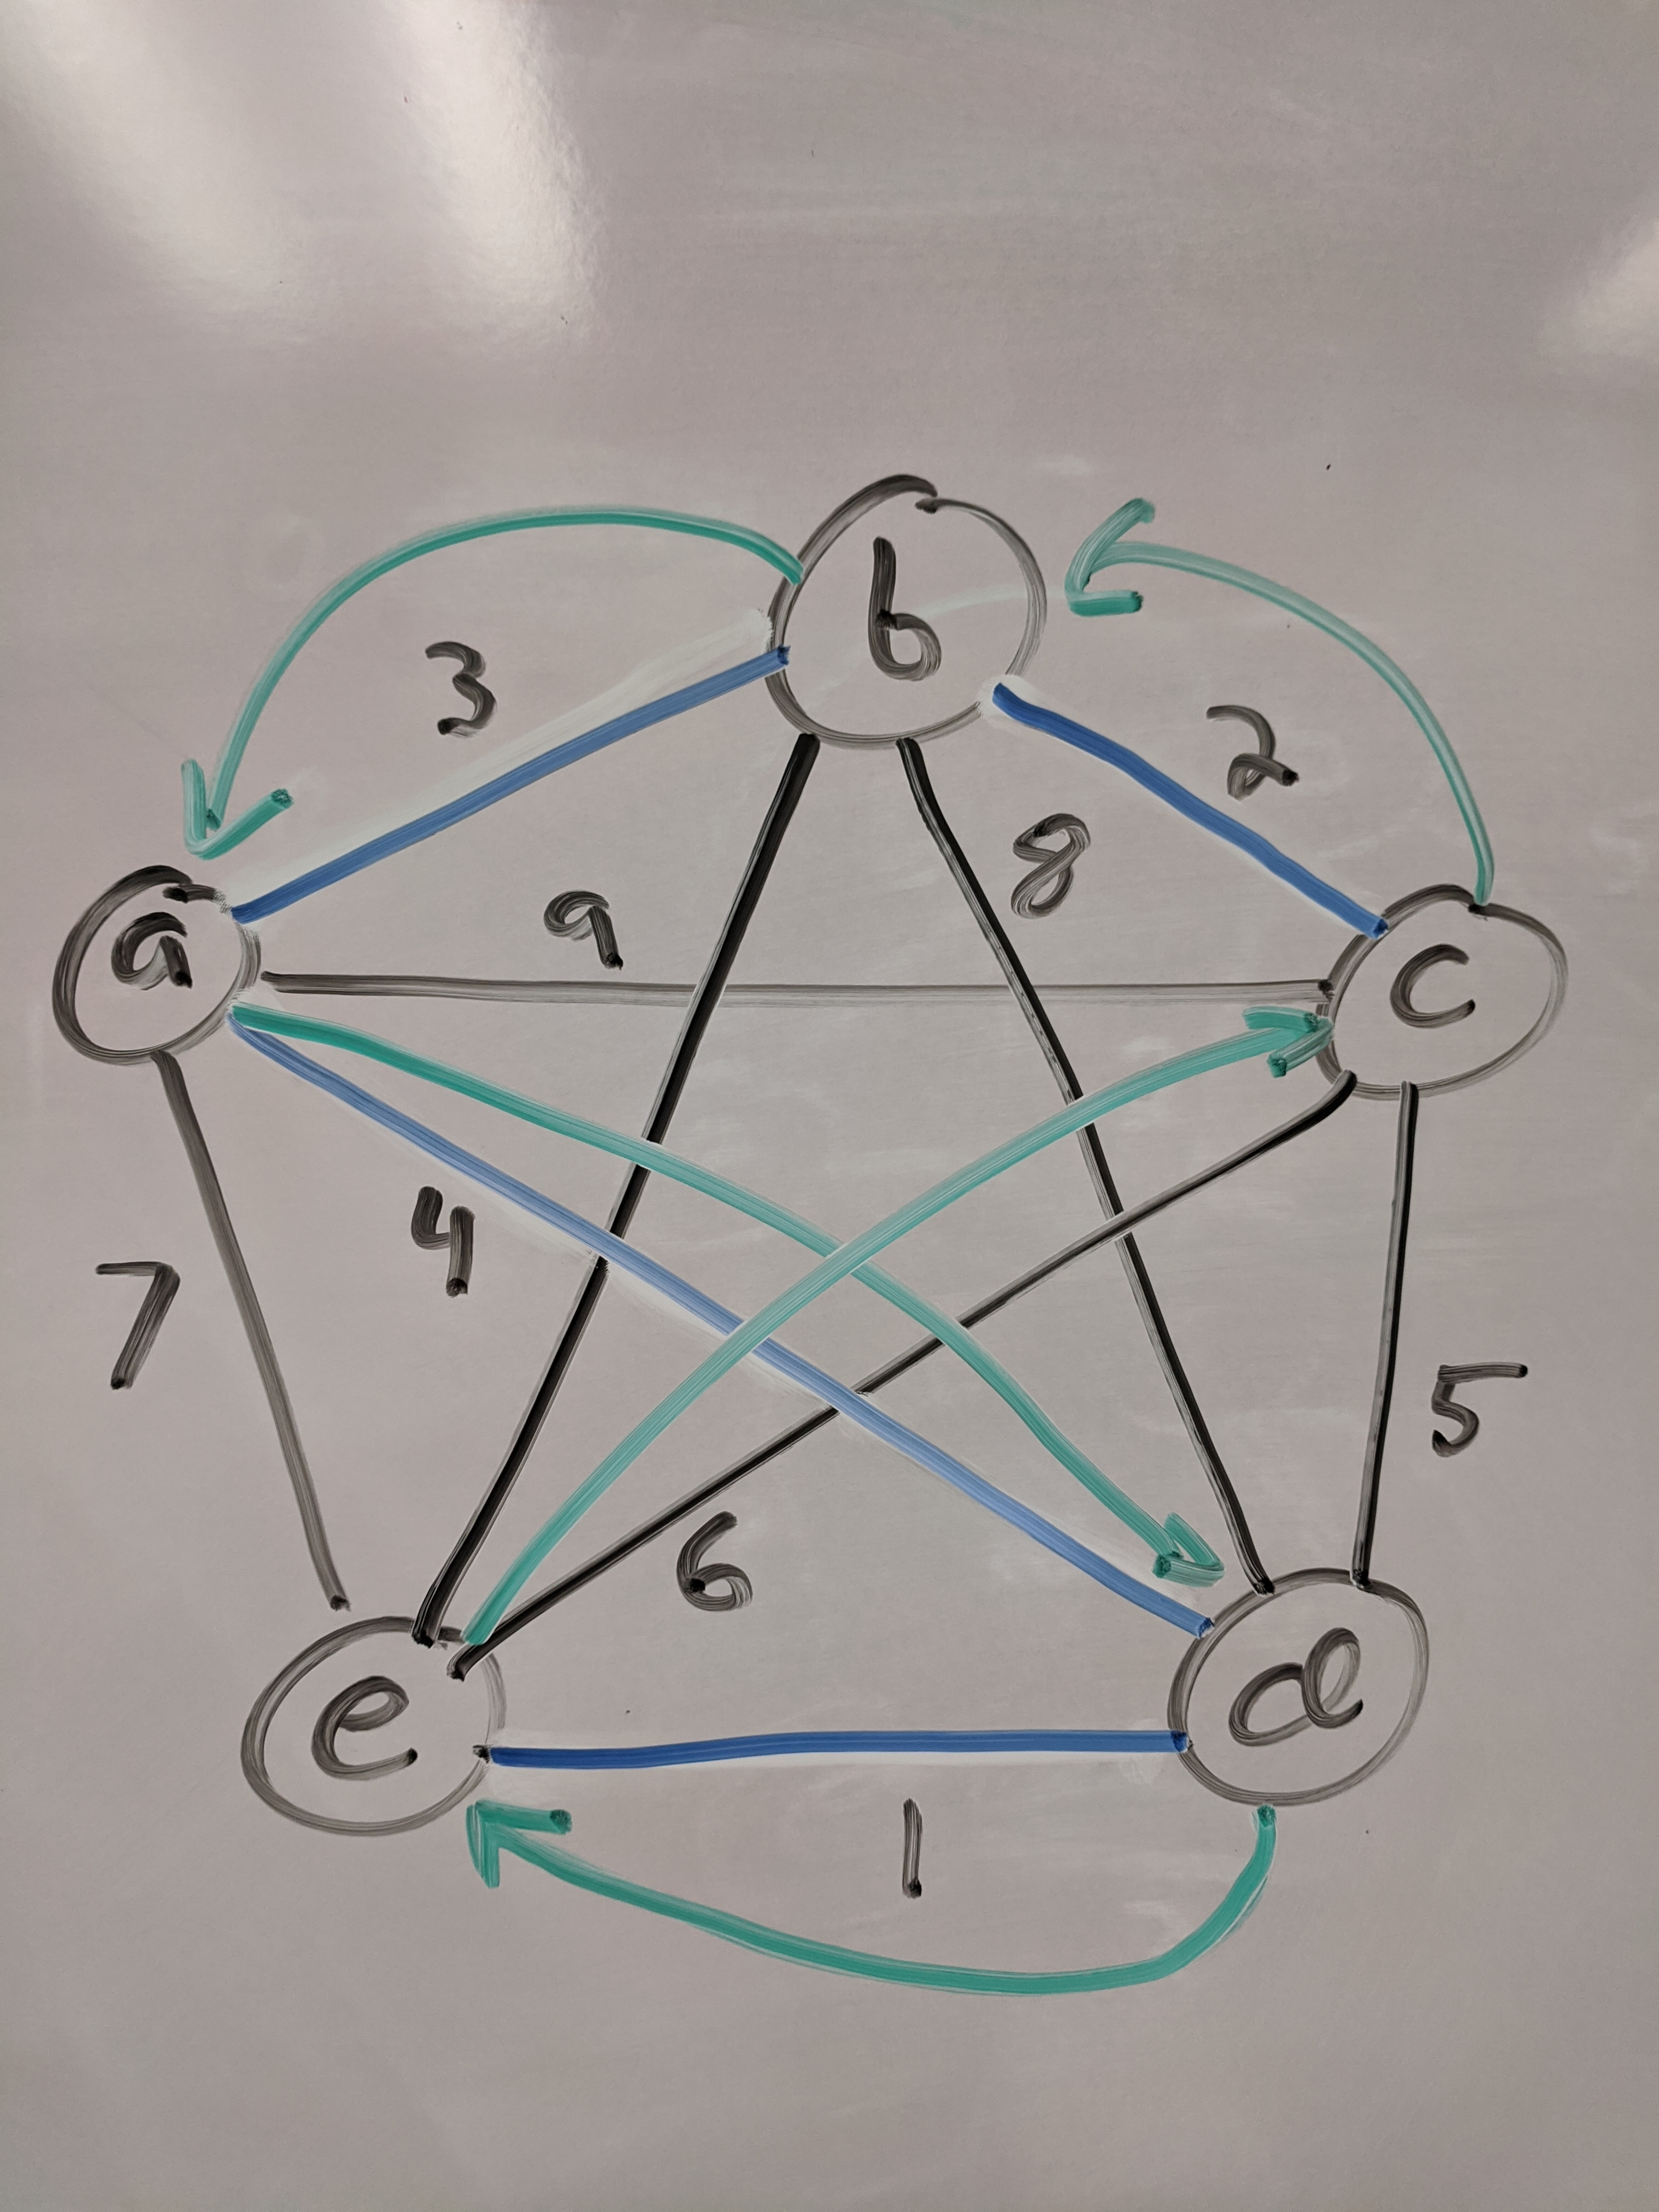
\includegraphics[height=160pt]{13-tspti-output.jpg}
    \end{center}
  \end{frame}
  
  \begin{frame} \frametitle{TSPTI Performance}
  \textbf{Lemma}: APPROX-TSPTI is a 2-approximation algorithm \\
  \textbf{Proof Sketch}:
  \begin{itemize}
    \item let $H^\star$ be an optimal Hamiltonian cycle for $G$
    \item (1) every spanning tree is one edge short of a cycle; and weights are nonnegative;
      so the weight of our tree $T$ obeys $w(T) \leq w(H^\star)$
    \item (2) a \emph{full tour} $W$ is the sequence of vertices in both a preorder and postorder
      tour, and has weight $w(W) = 2 w(T)$
    \item (3) combining (1) and (2), $w(W) \leq 2 w(H^\star)$
    \item (4) our $H$ is like $W$ with some vertices removed, so $w(H) \leq w(W)$
    \item combining (3) and (4),
      \[ w(H) \leq w(W) \leq 2 w(H^\star) \]
  \end{itemize}
  \end{frame}
  
  \begin{frame} \frametitle{Summary}
  Vertex cover:
  \begin{itemize}
    \item NP-complete
    \item exact exhaustive search alg. takes $\Theta(2^n m)$ time
    \item 2-approximate alg. takes $\Theta(n+m)$ time \stanza
  \end{itemize}
  
  TSP:
  \begin{itemize}
    \item NP-complete
    \item exact exhaustive search alg. takes $\Theta(n!)$ or $\Theta(2^m(n+m))$ time
    \item 2-approximate algorithm takes $O(m + n \log n)$ time
  \end{itemize}
  \end{frame}

\end{document}
